\lhead{\begin{tikzpicture}[remember picture, overlay]
    \node [anchor=100,inner sep=0] (imagenIZQUIERDA) at (current page header area.north){
\includegraphics[width=18cm]{img/Encabezado.PNG}};
    \end{tikzpicture}}
    \rhead{Flores-Antonio}
    \rfoot{\begin{tikzpicture}[remember picture, overlay]
    \node [anchor=140,inner sep=0] (imagenDERECHA) at (current page footer area.south){
\includegraphics[width=18cm]{img/Foot.PNG}};
    \end{tikzpicture}}
    %----------------------------------------------------------------------------------------
    \lfoot{ \thepage}
    % \renewcommand{\labelenumi}{\alph{enumi}.)} 
    %----------------------------------------------------------------------------------------
    %----------------------------------------------------------------------------------------
    %	TITLE SECTION
    %----------------------------------------------------------------------------------------
    
    \setlength{\droptitle}{-5\baselineskip} % Move the title up
    \title{\textbf{Estudio de tiempos y movimientos en el ensamble de un circuito electrónico utilizando diferentes métodos para su optimización }} % Article title
    
     \author{ 
     \textsc{Flores-Antonio, David Ricardo}\\ 
    %  Afiliación:
     \texttt{ Instituto Tecnológico de Querétaro } \\ 
     \texttt{Tecnológico Nacional de México} \\ 
     \texttt{Querétaro, México}\\ 
     \texttt{daroan13@gmail.com} 
     \and 
     \textsc{áNGELES-HURTADO, LUIS ALBERTO}\\ 
    %  Afiliación:
     \texttt{ Instituto Tecnológico de Querétaro } \\ 
     \texttt{ Tecnológico Nacional de México } \\ 
     \texttt{Querétaro, México}\\ 
     \texttt{alb3rto.ah@gmail.com} 
    }
    
    
    %----------------------------------------------------------------------------------------
    
    % \begin{document}
    
    % Print the title
    \maketitle
    \thispagestyle{fancy}
    
    %----------------------------------------------------------------------------------------
    %	ARTICLE CONTENTS
    %----------------------------------------------------------------------------------------
    
    % \section*{Resumen}
    % \textit{Palabras clave:}
    % El resumen (ancho de página) deberá contener entre 100 y 200 palabras tipo Adobe Devangari 11 puntos.
    
    \begin{abstract}
    \noindent 
    El resumen (ancho de página) deberá contener entre 100 y 200 palabras tipo Adobe Devangari 11 puntos.
    
    \end{abstract}
    % 
    % 
    \textbf{\textit{Palabras clave}}: {First keyword should be the corresponding to the research area according with the authors guide. Maximum of 6 keywords.}
    % \keywords{First keyword should be the corresponding to the research area according with the authors guide. Maximum of 6 keywords.}
    
    \section{Introducción}
    
% \begin{itemize}
%     \item Se debe exponer de manera concreta y en lenguaje sencillo : el tema, o lo(s) objeto (s) de estudio. 
%     \item Se deben de mencionar las metodologías más usadas muy brevemente. 
%     \item Se debe de señalar el avance en los últimos años.
%     \item Al final se debe hacer alusión al o lo(s) objetivos del proyecto de investigación.
%     \item Debe de tener Referencias científicas, URL, tesis, etc.
% \end{itemize}
% Define estudio de tiempos y movimientos
El estudio de tiempos y movimientos es una técnica de análisis utilizada en la ingeniería industrial y la gestión de operaciones para mejorar la eficiencia y productividad de los procesos laborales. Este estudio implica dos componentes principales: la medición del tiempo necesario para realizar cada tarea y el análisis de los movimientos realizados durante el trabajo. \cite{Estudiodetiempos}
% define que es ensamble
Un ensamblaje, en el contexto de la producción y la ingeniería, se refiere al proceso de unir o montar varias piezas o componentes individuales para crear un producto final completo. Este término es ampliamente utilizado en diversas industrias, especialmente en la manufactura y la electrónica, donde múltiples partes deben ser ensambladas para formar un dispositivo funcional. \cite{Ensamble}
% define que es un circuito electronico
Un circuito electrónico es una configuración de componentes eléctricos y electrónicos conectados entre sí mediante conductores, que permite el flujo de corriente eléctrica para realizar una función específica. Estos componentes pueden incluir resistencias, condensadores, diodos, transistores, y otros dispositivos que trabajan juntos para procesar señales, realizar cálculos, o controlar otros sistemas. \cite{Circuitoelectrico}
%define optimización
Optimizar hace referencia a la acción y efecto de optimizar. En términos generales, se refiere a la capacidad de hacer o resolver alguna cosa de la manera más eficiente posible y, en el mejor de los casos, utilizando la menor cantidad de recursos. \cite{optimizacion}
% define el metodo de tiempos predeterminados
Para poder realizar el siguiente trabajo utilizaremos el método de tiempos predeterminados, que es una técnica utilizada en el estudio de tiempos y movimientos para establecer estándares de tiempo mediante el uso de datos previamente recopilados y sistematizados sobre los tiempos necesarios para realizar movimientos y tareas básicas. Este método es ampliamente utilizado en la ingeniería industrial para mejorar la eficiencia operativa, planificar la producción y establecer objetivos de rendimiento.
% Al final se debe hacer alusión al o lo(s) objetivos del proyecto de investigación.
El objetivo general de este proyecto de investigación es optimizar el proceso de ensamblaje de circuitos electrónicos mediante el análisis detallado de tiempos y movimientos, con el fin de mejorar la eficiencia, reducir los tiempos de producción, minimizar costos y asegurar una alta calidad en el producto final. Esto incluye varios objetivos específicos, como identificar y eliminar movimientos innecesarios, asegurar que cada paso del proceso se realice de manera eficiente y con alta calidad, y aumentar la productividad implementando métodos más eficientes.
%
%
    \section{Justificación}

% \begin{itemize}
%     \item Se debe de describir lo que se requiere, lo que se necesita o lo que se demanda en la actualidad con un enfoque global pero terminar con menciones a temas locales o nacionales.
%     \item Debe de tener Referencias científicas, URL, tesis, etc.
% \end{itemize}
% 
% Cuantos tipos de manufactura existen?
La manufactura se refiere al proceso de convertir materias primas en productos terminados a través del uso de herramientas, mano de obra, maquinaria y procesos químicos. Existen varios tipos de manufactura, cada uno adecuado para diferentes tipos de productos y necesidades de producción. Cada tipo de manufactura tiene sus propias ventajas y desventajas, y su elección depende de factores como el tipo de producto, la cantidad de producción, los costos, la flexibilidad requerida y la tecnología disponible. \cite{Manufactura}
% Cuantas empresas de manufactura existen en Mundo?
Determinar la cantidad exacta de empresas de manufactura en todo el mundo es un desafío debido a la variedad de definiciones y la constante evolución del sector.
Según un informe de McKinsey, el sector manufacturero representa aproximadamente el 16 del PIB global y el 14 del empleo mundial. En resumen, aunque es difícil proporcionar una cifra exacta, el sector manufacturero es vasto y en expansión, con millones de empresas a nivel mundial contribuyendo significativamente a la economía global. \cite{Empresas}
    % 
    % 
    \section{Descripción del problema}
    % \begin{itemize}
%     \item Se debe describir la desviación o diferencia del ``es'' con respecto al ``debe ser''.
%     \item Se debe hacer alusión a la incógnita científica*.
%     \item Debe de tener Referencias científicas, URL, tesis, etc.
% \end{itemize}
% \textbf{*La incógnita científica es el elemento cuya solución incrementa el conocimiento científico.}
% 
% 
El Instituto Tecnológico de Querétaro (ITQ) es una Institución de Educación Superior y Posgrado que forma profesionales mediante un modelo educativo integral de calidad, que garantiza una formación técnica humanística, con capacidad para investigar y aplicar tecnología con impacto en el desarrollo de la sociedad. El Instituto Tecnológico de Querétaro  tiene como objetivo principal formar profesionistas competentes a nivel nacional e internacional, comprometidos con el desarrollo sustentable y la mejora continua de la calidad de vida. Los egresados deberán
contar con los siguientes atributos:
\begin{enumerate}
    \item Diseña, mejora e integra sistemas productivos de bienes y servicios aplicando tecnologías para su optimización.
    \item Diseña, implementa y mejora sistemas de trabajo para elevar la productividad.
    \item Implanta sistemas de calidad utilizando métodos estadísticos para mejorar la competitividad de las organizaciones.
    \item Administra sistemas de mantenimiento en procesos de bienes y servicios para la optimización en el uso de los recursos.
    \item Gestiona sistemas de seguridad, salud ocupacional de manera sustentable, en sistemas productivos de bienes y servicios atendiendo los lineamientos legales.
    \item Formula, evalúa y gestiona proyectos de inversión, sociales y de transferencia de tecnología para el desarrollo regional.
\end{enumerate} 
El nivel de educación en las universidades puede verse afectado por una variedad de factores que interactúan de manera compleja. La calidad del profesorado es fundamental; si los docentes no están bien calificados o motivados, esto puede impactar negativamente en la educación. Además, la falta de recursos e infraestructura adecuados, como laboratorios, bibliotecas, tecnología y espacios apropiados, limita el aprendizaje y la investigación. Una infraestructura deficiente puede también desmotivar tanto a estudiantes como a profesores.

El plan de estudios juega un papel crucial, ya que un currículo desactualizado o mal diseñado puede no preparar adecuadamente a los estudiantes para los desafíos del mundo moderno. Es esencial que los programas académicos se mantengan actualizados y sean pertinentes a las demandas del mercado laboral y la sociedad. La gestión y administración de la universidad también influyen; una administración ineficiente puede llevar a una mala asignación de recursos, problemas burocráticos y desmotivación.
el nivel de educación en las universidades es el resultado de una interacción compleja de múltiples factores. La calidad del profesorado, la disponibilidad de recursos e infraestructura, la actualización y pertinencia del plan de estudios, la eficiencia de la gestión y administración, y el financiamiento adecuado son esenciales para asegurar una educación de alta calidad. Además, la accesibilidad y equidad, el fomento de la investigación, un ambiente académico positivo, la participación activa y el compromiso de los estudiantes, así como políticas gubernamentales efectivas, juegan roles cruciales. Abordar estos elementos de manera integral y con un enfoque en la mejora continua es fundamental para elevar y mantener el nivel educativo en las universidades, garantizando así la formación de profesionales competentes y comprometidos con el desarrollo sostenible y el bienestar social.
%
%
    \section{Fundamentación teórica}
    
%Es la parte medular y de mayor discusión, deberá ser la fundamentación de la hipótesis, por tanto se deberá señalar claramente la razón de la suposición y fundamentación de la misma. Únicamente referencias científicas.
%\begin{itemize}
        %\item Se debe de retomar el tema que se planteo en la introducción, pero ahora profundizando para clarificar la incógnita científica y se pueda plantear la hipótesis.
        %\item Se debe de retomar la descripción del problema, pero ahora a profundidad del (los) objeto(s) de estudio. 
        %\item Se debe de profundizar en las metodologías que se ha usado para el estudio del tema.
       % \item Referencias solo de artículos y libros científicos.
    %\end{itemize}
% 
% 
% Cuales son las revoluciones industriales que ha vivido la humanidad?
% A lo largo de la historia del hombre las técnicas manuales para elaborar herramientas y mejorar la caza y la calidad de vida fueron fundamentales para la supervivencia.
% La revolución industrial han cambiado las fuentes de energía básicas y los medios de comunicación para desplazar mercancías, personas e información.
El estudio de tiempos y movimientos es una técnica fundamental en la ingeniería industrial que busca mejorar la eficiencia de los procesos productivos. Este proyecto se enfoca en analizar y optimizar el proceso de ensamble de circuitos electrónicos, crucial en la industria de la electrónica, donde la precisión y la eficiencia son esenciales para la competitividad y la satisfacción del cliente. La fundamentación teórica del proyecto se basa en principios de gestión de operaciones, ingeniería de métodos, ergonomía y análisis de sistemas.
La ingeniería de métodos, basada en los estudios pioneros de Frederick Taylor y Frank y Lillian Gilbreth, busca mejorar los métodos de trabajo mediante el análisis sistemático de los procesos. Barnes (2018) define el estudio de métodos como una técnica para aumentar la eficiencia mediante la simplificación del trabajo y la reducción del tiempo requerido para completar tareas. En este contexto, se analizan las operaciones manuales y automatizadas en el ensamble de circuitos, buscando formas de simplificar y estandarizar el trabajo.
Para la optimización del proceso de ensamble de circuitos electrónicos, se pueden emplear varias metodologías:
\begin{itemize}
    \item\textbf{Lean Manufacturing:} Según Womack y Jones (2003), Lean Manufacturing busca eliminar desperdicios y mejorar el flujo de trabajo. Aplicar técnicas Lean, como el mapeo de flujo de valor y la mejora continua (Kaizen), puede reducir tiempos de ciclo y aumentar la eficiencia del ensamble.\cite{Lean}
    \item\textbf{Six Sigma:} Definido por Pande, Neuman y Cavanagh (2000), Six Sigma utiliza un enfoque basado en datos para reducir la variabilidad y mejorar la calidad del proceso. Aplicar el ciclo DMAIC (Definir, Medir, Analizar, Mejorar y Controlar) puede identificar y eliminar defectos en el proceso de ensamble. \cite{Sixsigma}
    \item\textbf{Tecnologías de Automatización:} La implementación de tecnologías avanzadas, como la robótica y la inteligencia artificial, puede automatizar tareas repetitivas y aumentar la precisión. Según Groover (2016), la automatización mejora la consistencia y reduce el tiempo de ciclo. \cite{Tecnologias}
\end{itemize}
El estudio de tiempos y movimientos en el ensamble de circuitos electrónicos utilizando diferentes métodos de optimización se fundamenta en principios de gestión de operaciones, ingeniería de métodos, ergonomía y análisis de sistemas. Aplicar estas teorías y metodologías puede mejorar significativamente la eficiencia, la calidad y la seguridad del proceso de ensamble. Este enfoque integral permitirá identificar y eliminar ineficiencias, optimizando el uso de recursos y mejorando la competitividad en la industria electrónica.
% 
% 
\section{Hipótesis}
 % Es la suposición con fundamento científico relativa a la solución del problema, necesidad o de cómo se aprovecha la oportunidad con la incógnita científica y se fundamenta con: 1. Una suposición (en afirmativo o negativo) y ésta deberá vincularse con:
% 2. La fundamentación científica que deberá ser precisa 3. Una entidad de comparación para probar la suposición y
% 4. La variable con que se califica o cuantifica la comparación o se prueba la hipótesis.
% 
% 
% 
% 
% \begin{itemize}
%     \item Se debe de identificar claramente la suposición científica
%     \item Se debe de identificar claramente el fundamento científico
%     \item Se debe identificar claramente la variable de respuesta
%     \item Se debe identifican claramente las realidades o modelos contrastantes
%     \item Se debe de establecer las variables asociadas, explicativas o que tienen relación funcional con la variable de respuesta
% \end{itemize}
Desarrollar un proyecto integrador en la materia de estudio del trabajo II implementando todos los temas vistos en la clase, incrementará las habilidades del estudiante, logrando plantear nuevos proyectos desde cero al determinar el tiempo estándar en el ensamble de un circuito electrónico.
% 
%  
\section{Objetivo}

% Precisar la acción necesaria para probar la hipótesis. Dicha acción se establece mediante el uso de verbos activos y en infinitivo.
% 
% 
% \begin{itemize}
%     \item Se debe establecer que se pretende probar la hipótesis
% \end{itemize}
% 
%
El alumno diseñará, mejorará e integrará sistemas productivos de bienes y servicios aplicando tecnologías para su optimización.
Diseñará, implementará y mejorará sistemas de trabajo para elevar la productividad.
En un plazo menor a seis meses y se plasmara en un proyecto integrador.
%
%
\subsection{Objetivos específicos }

  % \begin{itemize}
%     \item Se debe establecer como un conjunto de acciones comunes para lograr el objetivo general
%     \item Se debe establecer como etapas para lograr el objetivo general
% \end{itemize}

% Son actividades orientadas al cumplimiento del objetivo general. Se establecen con verbos activos en infinitivo. Son parte de la acción encaminada a probar la hipótesis. Éstos deben ser precisos, y en lo posible evitar aspectos metodológicos.
% 
%
\begin{itemize}
    \item Desarrollar una guía de emergencia para analizar la instalación en la que se llevo acabo la experimentación.
    \item Analizar los métodos, materiales, herramientas e instalación utilizada o que se ha de utilizar en la ejecución del ensamble de un circuito electrónico.
    \item Se establecerá la forma más económica de realizar el trabajo.
    \item Normalizar los métodos, materiales, herramientas e instalaciones.
    \item Determinar exactamente el tiempo necesario para que una persona competente realice el trabajo con una marcha normal.
\end{itemize} 
    % 
    % 
\section{Metodología}

El presente trabajo de investigación se llevó a cabo mediante la observación directa y el análisis estadístico de los datos recolectados.
El estudio y la recolección de datos se realizaron en la ciudad de Querétaro, específicamente en las instalaciones del Instituto Tecnológico de Querétaro (ITQ).
La experimentación se desarrolló durante el período comprendido entre febrero y mayo de 2024.
Se eligió el ensamblaje de una tarjeta electrónica como caso de estudio, empleando software de diseño asistido por computadora para definir la estructura en todos sus niveles. Además, se establecieron los límites de potencia y control necesarios para desarrollar la arquitectura adecuada, y se seleccionó la mejor opción para su implementación final. 
En la primera fase de la experimentación, se grabaron dos muestras continuas con una cámara de vídeo de celular, y luego se aplicaron varias metodologías para determinar el tiempo de ciclo y el tiempo estándar.

\subsection{Desarrollo de la guía de plan de Emergencia}

Un plan de emergencia es un conjunto de procedimientos y acciones predefinidas diseñadas para mitigar, responder y recuperarse de situaciones de emergencia o desastres.\cite{Plan}
\newline
Su objetivo principal es proteger la vida humana, minimizar daños y asegurar una recuperación rápida y efectiva. Un plan de emergencia abarca una variedad de escenarios, incluyendo desastres naturales, incidentes tecnológicos, y emergencias causadas por el hombre.
%
%
\subsection{Análisis de los métodos, materiales, herramientas e instalación utilizada en la ejecución del ensamble de un circuito electrónico}


\subsubsection{Planeación}

%Asegúrate de conocer siempre tu objetivo.
%Asegúrate de contar con los documentos (formatos, procedimientos, etc).
%
%
Para iniciar este trabajo es esencial planificar todas las actividades, especialmente el manejo del material nuevo que requiere extremo cuidado. Se debe generar una lista de pasos sencilla y clara para que los operadores realicen su labor adecuadamente. Es importante usar herramientas como las 5S para asegurar un orden riguroso en la implementación de las metodologías. Además, es necesario recopilar datos para crear un plan de emergencia, incluyendo conocimiento métrico de las áreas cercanas y materiales de protección en el entorno del área de trabajo.
    
\subsubsection{5´s}

Las 5's es una metodología de gestión de calidad originada en Japón que busca mejorar el entorno de trabajo a través de la organización y la estandarización. Su nombre proviene de cinco palabras japonesas que comienzan con la letra "S", y cada una representa un paso fundamental del proceso. La implementación de las 5's puede mejorar la eficiencia, reducir desperdicios, y crear un ambiente de trabajo más seguro y organizado. \cite{5´s}
\newline
Consiste en cinco principios: Seiri (Clasificación), que elimina elementos innecesarios; Seiton (Orden), que organiza los elementos necesarios de manera lógica; Seiso (Limpieza), que mantiene el área de trabajo limpia; Seiketsu (Estandarización), que establece procedimientos para mantener la clasificación, orden y limpieza; y Shitsuke (Disciplina), que fomenta la adherencia continua a estos estándares.
\newline
\begin{enumerate}
     \item\textbf{Clasificación (Seiri):}  
        Se identificará y clasificarán todos los componentes y herramientas para el ensamble del circuito eléctrico. Se eliminará del área de trabajo cualquier cosa que no sea necesaria, así cómo componentes defectuosos y herramientas que no sean relevantes.
        \item\textbf{Orden(Seiton):}Se colocarán los componentes, herramientas en lugares designados y etiquetados para que sean fáciles de encontrar y acceder ahorrando tiempo en la búsqueda.
        \item\textbf{Limpieza (Seiso):} Es indispensable localizar y eliminar la suciedad del puesto de trabajo, así como su correcto mantenimiento. Disponer de un estándar adecuado de limpieza y organización repercute directamente en la motivación del personal, además de reducir en gran medida los accidentes y lesiones.
        \item\textbf{Estandarización (Seiketsu):} Se desarrollaran procedimientos estandarizados para la clasificación, organización y limpieza. Se sugiere crear listas de verificación y hacer las correcciones pertinentes al manual de procedimientos.
        \item\textbf{Disciplina (Shitsuke):} Se capacitará y motivará al operador para que siga los procedimientos establecidos, realizando supervisiones regulares para asegurar el cumplimiento de estas.
        
    \end{enumerate}
%
%
\subsubsection{Desarrollo del sistema de tiempos predeterminado}

Los tiempos predeterminados, son una reunión de tiempos estándares válidos asignados a movimientos fundamentales y grupos de movimientos que no pueden ser evaluados de forma precisa con los procedimientos ordinarios para estudio de tiempos con cronómetro. Éstos son el resultado de estudiar una gran muestra de operaciones diversificadas con un dispositivo de medición de tiempo, como una cámara de cine o de video grabación capaz de medir lapsos muy pequeños de tiempo(Wygant 2003). Entre los más comunes están: MTM (Methods Time Measurement), MOST (Maynard Operation Sequence Tecnique), WORK FACTOR entre otros. \cite{Tiempospredeterminados}
\newline
Los sistemas de tiempos predeterminados Son una colección de tiempos de movimientos básicos. Se asignan a los movimientos fundamentales y a grupos de movimientos que no es posible evaluar con precisión mediante los procedimientos normales de estudio de tiempos con cronometro. Son resultado del estudio de una muestra grande de diversas operaciones con un dispositivo de tiempos como una cámara de película o de video-grabación capaz de medir elementos muy cortos. \cite{Sistemadetiempos}


\begin{figure}[H]
        \centering
        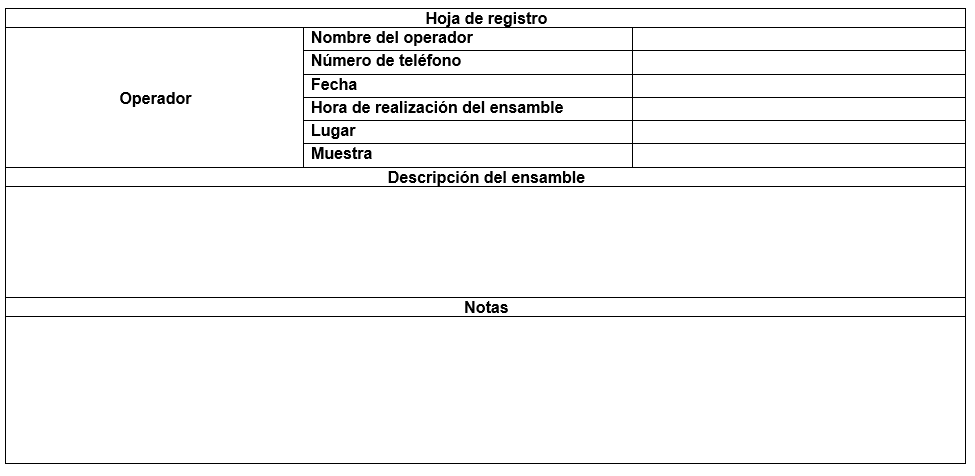
\includegraphics[trim = {0mm 0mm 0mm 0mm},clip,scale=0.2]{10/Img/hojaRegistro.png}
        \caption{Hoja de registro}
        \label{hojaRegistro}
\end{figure}

\textbf{MTM}

El MTM es un procedimiento que analiza cualquier operación manual o método por los movimientos básicos necesarios para ejecutarlos, asignando a cada movimiento un tiempo tipo predeterminado que se define por la índole del movimiento y las condiciones en que se efectúa. Procedimiento para el empleo del MTM. \cite{MTM}
\begin{enumerate}
    \item Determinar los micromovimientos básicos que deben de utilizarse en la operación que se estudia.
    \item Sumar el valor del tiempo dados por las tablas de datos de la MTM para cada uno de dichos movimientos.
    \item Conceder el suplemento por fatiga, retrasos personales y retrasos inevitables en caso de ser necesario.
    \item Los datos se deben de registrar en TMU.
\end{enumerate}

\begin{figure}[H]
        \centering
        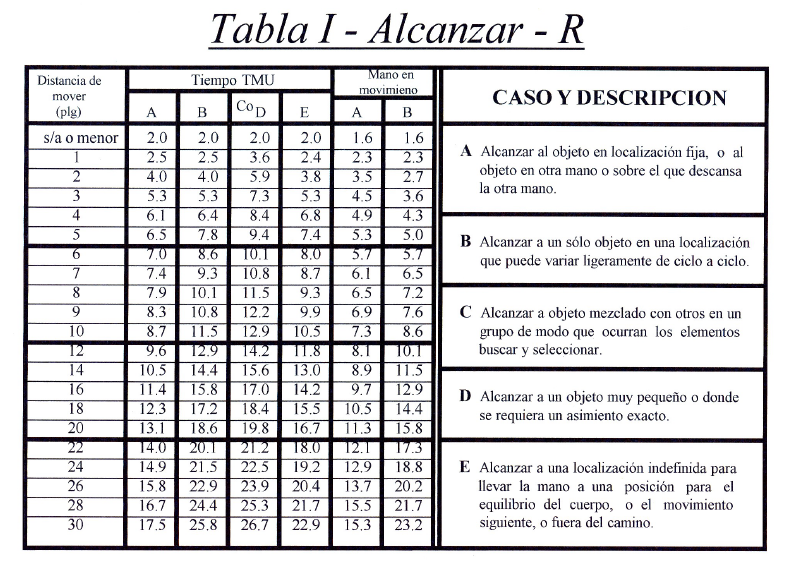
\includegraphics[trim = {0mm 0mm 0mm 0mm},clip,scale=0.2]{10/Img/tabla1.png}
        \caption{Tabla de tiempos TMU para el movimiento Alcanzar}
        \label{tabla1}
\end{figure}

\begin{figure}[H]
        \centering
        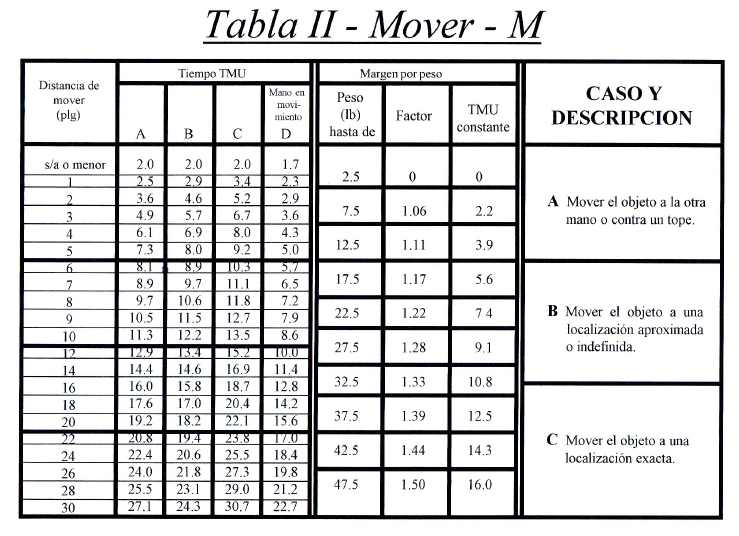
\includegraphics[trim = {0mm 0mm 0mm 0mm},clip,scale=0.2]{10/Img/tabla2.png}
        \caption{Tabla de tiempos TMU para el movimiento Mover}
        \label{tabla2}
\end{figure}

\begin{figure}[H]
        \centering
        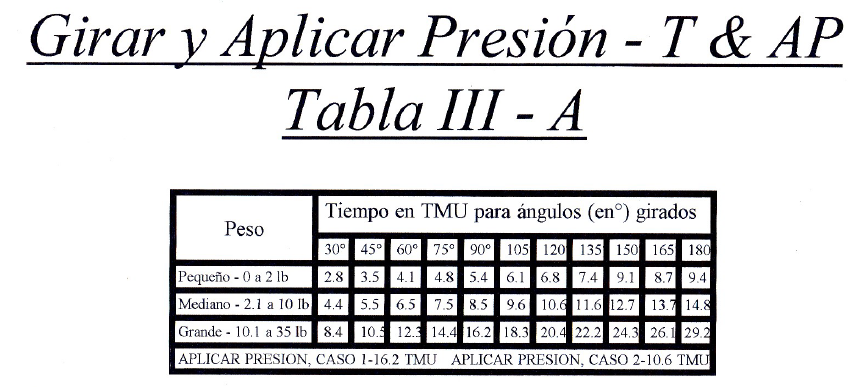
\includegraphics[trim = {0mm 0mm 0mm 0mm},clip,scale=0.2]{10/Img/tabla3A.png}
        \caption{Tabla de tiempos TMU para el movimiento Girar}
        \label{tabla3A}
\end{figure}

\begin{figure}[H]
        \centering
        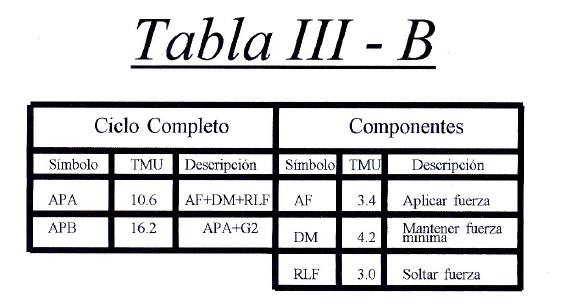
\includegraphics[trim = {0mm 0mm 0mm 0mm},clip,scale=0.2]{10/Img/tabla3B.png}
        \caption{Tabla de tiempos TMU para el movimiento Aplicar Presión}
        \label{tabla3B}
\end{figure}

\begin{figure}[H]
        \centering
        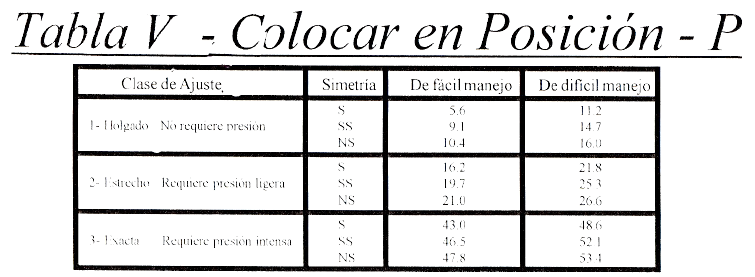
\includegraphics[trim = {0mm 0mm 0mm 0mm},clip,scale=0.2]{10/Img/tabla5.png}
        \caption{Tabla de tiempos TMU para el movimiento Colocar}
        \label{tabla5}
\end{figure}

\begin{figure}[H]
        \centering
        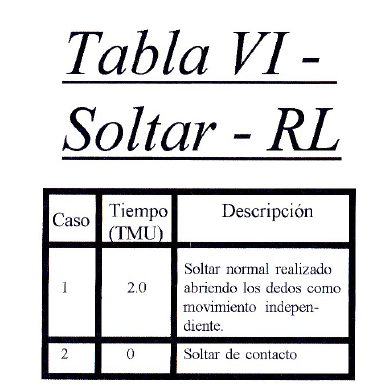
\includegraphics[trim = {0mm 0mm 0mm 0mm},clip,scale=0.2]{10/Img/tabla6.png}
        \caption{Tabla de tiempos TMU para el movimiento Soltar}
        \label{tabla6}
\end{figure}
%
%
\subsubsection{Desarrollo del muestreo del trabajo}

El muestreo de trabajo es una técnica que se utiliza para investigar las proporciones del tiempo total dedicada a las diversas actividades que componen una tarea, actividades o trabajo, mediante muestreo estadístico y observaciones aleatorias, el porcentaje de aparición de determinada actividad. Los resultados del muestreo sirven para determinar tolerancias o márgenes aplicables al trabajo, para evaluar la utilización de las máquinas y para establecer estándares de producción entre otras aplicaciones. \cite{Muestreodetrabajo}
%
%
\subsubsection{Corrección por balanceo de procesos}

La línea de producción es reconocida como la principal forma de producir grandes cantidades de elementos normalizados a costos bajos.

El Balanceo de Líneas de Ensamble consiste en agrupar actividades u operaciones que cumplan con el tiempo de ciclo determinado con el fin de que cada línea de producción tenga continuidad, es decir que en cada estación o centro de trabajo, cuente con un tiempo de proceso uniforme o balanceado, de esta manera las líneas de producción pueden ser continuas y no tener cuellos de botella.

En su estado más refinado, la producción en línea es una disposición de áreas de trabajo en el cual las operaciones consecutivas están colocadas inmediata y mutuamente adyacentes, en donde el material se mueve continuamente y a un ritmo uniforme a través de una serie de operaciones equilibradas que permiten efectividad simultánea en todos los puntos, moviéndose el producto hacia el fin de su elaboración a lo largo de un camino razonable directo. Este total refinamiento en el proceso no es, sin embargo, absolutamente necesario. \cite{Balanceodelineas}
%
%
\subsubsection{Datos estándar continuos y discretos}

Los datos estándar son una colección de tiempos bien definidos para elementos de trabajo, los cuales se obtienen mediante la medición de trabajo, que se organizan y definen en varios niveles de detalle según se requiera: movimientos, elementos o tarea; codificados en forma tabular o gráfica, o algebraica cuando se incluyen elementos variables. Cuando los datos estándar se identifican claramente, son de gran utilidad para establecer estándares de trabajo. Los datos estándar pueden ser definidos como el tiempo tipo o estándar requerido para la ejecución de una parte específica de trabajo. \cite{Datosestandar}
\newline
Los datos estándar continuos se refieren a datos cuantitativos que pueden tomar cualquier valor dentro de un rango continuo y que se utilizan como referencia para evaluar y comparar el rendimiento de procesos o tareas en un entorno de trabajo. Estos datos son fundamentales en estudios de tiempo y movimiento, análisis de eficiencia y otros contextos en ingeniería industrial y administración.
\newline
Los datos estándar discretos se refieren a datos que pueden tomar un conjunto finito o contable de valores específicos. Estos datos son fundamentales en varios contextos del estudio del trabajo, la ingeniería industrial y la gestión de operaciones.
%
%
\subsection{Diseño de la forma más económica de realizar el trabajo}   

Los estudios que llevaremos a acabo nos proporcionaran información valiosa sobre las actuales prácticas de ensamblaje y los factores que contribuyen a la eficiencia y productividad del proceso. Analizando estos datos en profundidad, identificaremos diversas áreas donde se pueden implementar mejoras significativas. Por ello, nos proponemos diseñar y adoptar un nuevo enfoque para el ensamblaje, enfocado en optimizar cada etapa del proceso.
%    
%   
\subsection{Normalización de los métodos, materiales, herramientas e instalaciones}    

En nuestra práctica, es fundamental conocer cada parte del ensamblaje. Como operarios, esto facilita nuestro trabajo al familiarizarnos con las piezas utilizadas. Como analistas, debemos examinar cada parte, medida y material para mejorar nuestro método y cumplir con el objetivo del estudio del trabajo: encontrar una forma más económica y estandarizar herramientas, materiales e instalaciones. Por eso, es necesario listar cada parte del ensamblaje para mantener una secuencia ordenada durante el estudio.

\begin{figure}[H]
    \centering
    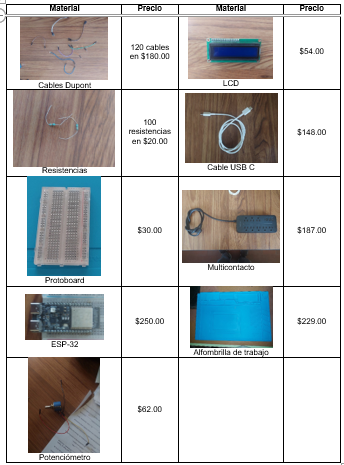
\includegraphics[scale=0.4]{10/Img/tablaMaterial.png}
    \caption{Tabla Materiales}
    \label{fig:tablaMaterial.png}
\end{figure}

Cada uno de los materiales se deben medir, tocar, oler y todo lo necesario para a partir de esto, plasmarlos en algún programa asistido por computadora especificando las medias de cada uno, en este caso se utilizó Solid Works en la versión 2019. Es necesario describirlos en su totalidad.

\textbf{Alfombrilla de trabajo}

Una alfombrilla de trabajo de silicona es una superficie protectora y multiusos fabricada con silicona, un material sintético conocido por su flexibilidad, resistencia al calor y propiedades antiadherentes. Estas alfombrillas se utilizan habitualmente en diversos entornos, tanto domésticos como profesionales, para proteger las superficies de trabajo, organizar herramientas y utensilios, y facilitar diversas tareas. \cite{Alfombrilla}

Características principales de las alfombrillas de trabajo de silicona:

\begin{itemize}
    \item\textbf{Flexibles:} Se pueden doblar, enrollar y adaptar fácilmente a diferentes espacios de trabajo.
    \item\textbf{Resistentes al calor:} Soportan altas temperaturas, lo que las hace ideales para su uso en cocinas y talleres.
    \item\textbf{Antiadherentes:} Repelen líquidos y derrames, protegiendo las superficies de trabajo subyacentes.
    \item\textbf{Fáciles de limpiar:} Se pueden lavar con agua y jabón o meterse en el lavavajillas.
    \item\textbf{Antiestáticas:} Algunos modelos disipan la electricidad estática, protegiendo componentes electrónicos sensibles.
\end{itemize}

\begin{figure}[H]
        \centering
        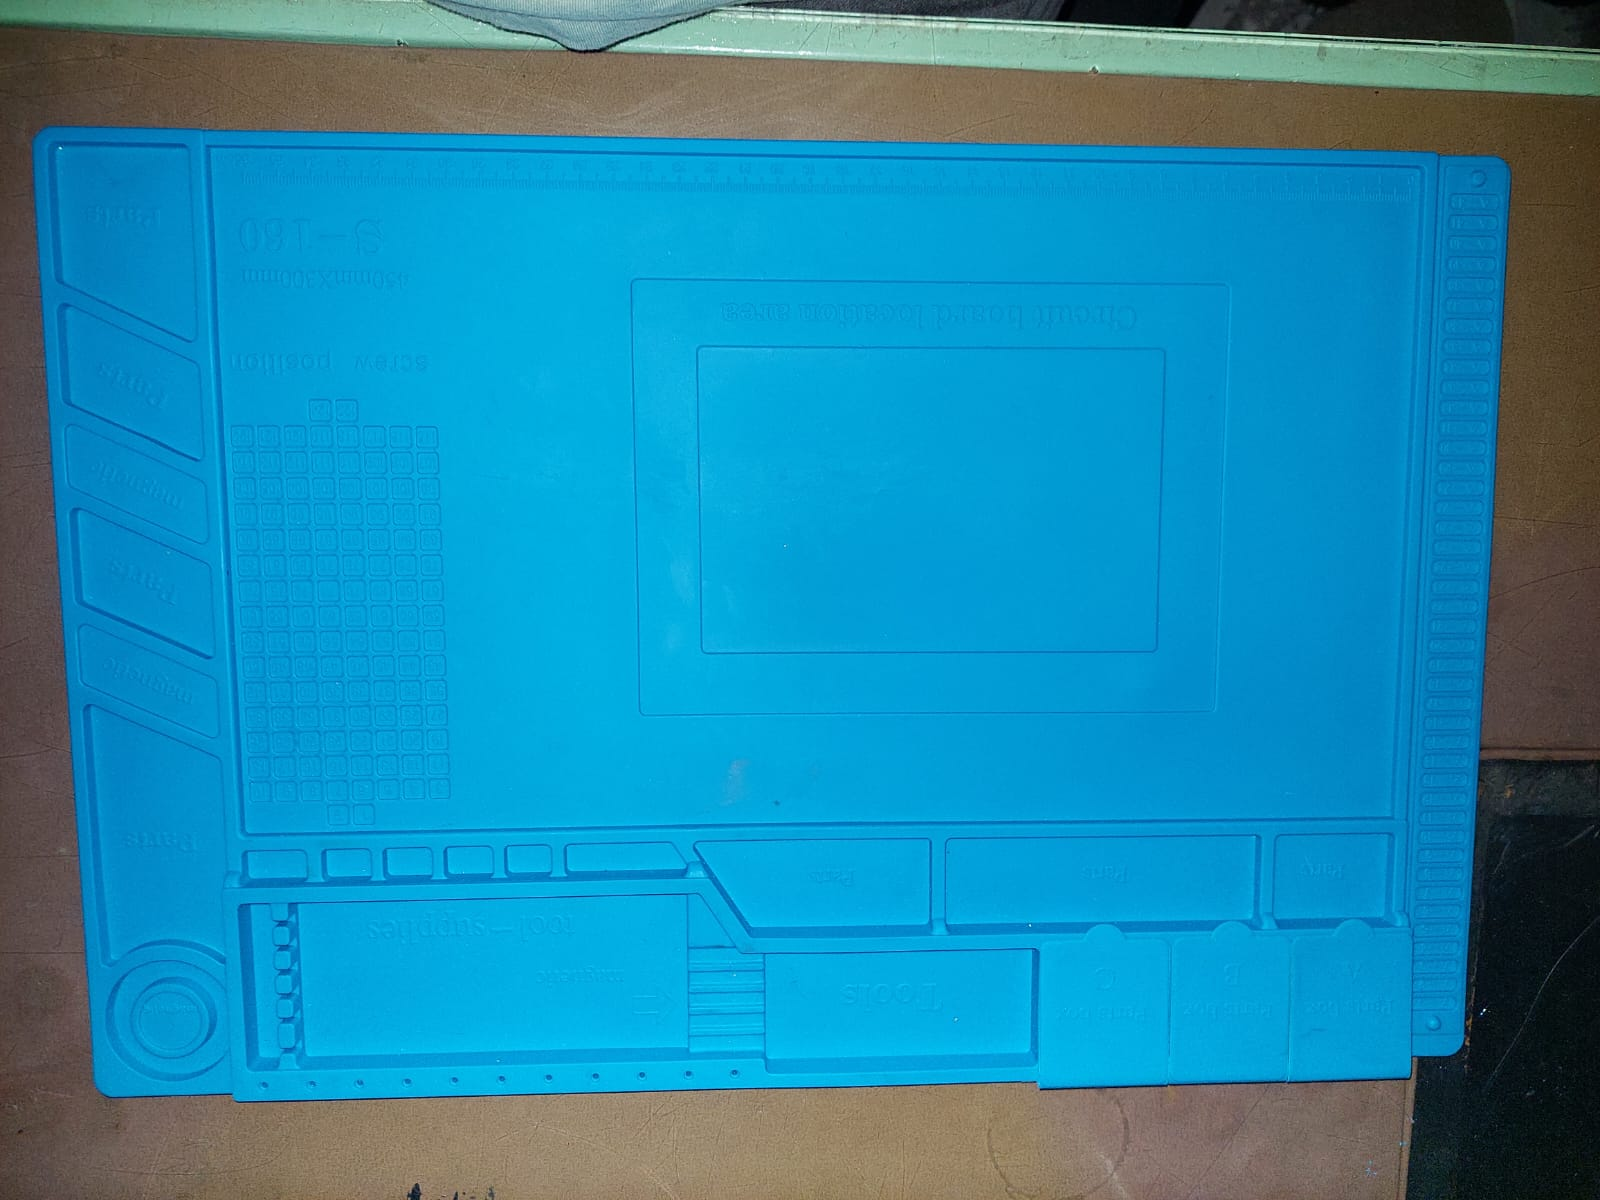
\includegraphics[trim = {0mm 0mm 0mm 0mm},clip,scale=0.2]{10/Img/alfombrilla.jpg}
        \caption{Alfombrilla de Trabajo}
        \label{añfombrilla}
    \end{figure}

\textbf{Protoboard}

Una protoboard, también conocida como placa de pruebas o placa de inserción, es una herramienta utilizada para construir circuitos electrónicos de forma temporal y experimental. Consiste en una base de plástico aislante con orificios interconectados por tiras metálicas conductoras, siguiendo patrones de líneas. Los componentes electrónicos, como resistencias, condensadores, transistores y circuitos integrados, se insertan en estos orificios y se conectan eléctricamente entre sí mediante los cables.

Las protoboards son una herramienta valiosa para los aficionados a la electrónica, estudiantes, ingenieros e inventores, ya que permiten construir y probar circuitos rápidamente y sin necesidad de soldar. Esto las hace ideales para el prototipado de nuevos diseños, la experimentación con diferentes componentes y circuitos, y la depuración de problemas. \cite{Protoboard}

\begin{figure}[H]
        \centering
        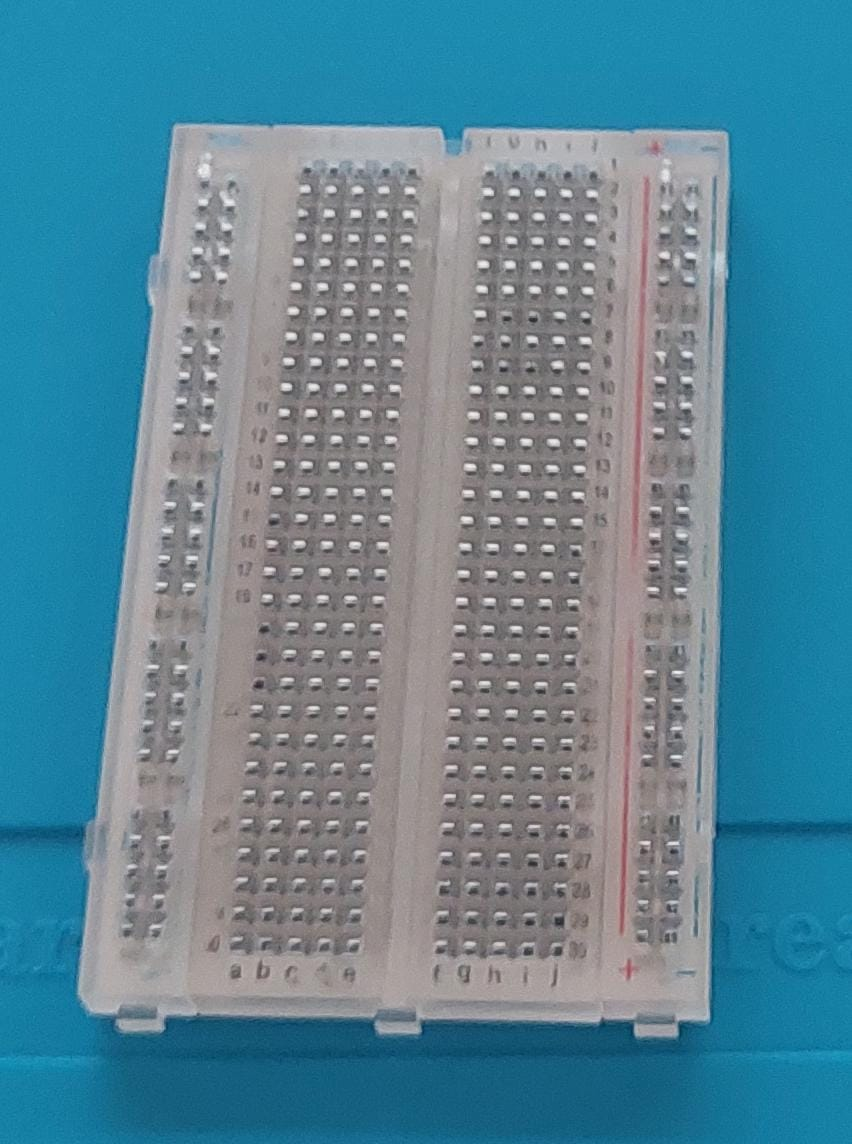
\includegraphics[trim = {0mm 0mm 0mm 0mm},clip,scale=0.2]{10/Img/protoboard.jpg}
        \caption{Protoboard}
        \label{Protoboard}
    \end{figure}

\textbf{LCD}

LCD, sigla del inglés Liquid Crystal Display, en español Pantalla de Cristal Líquido, es una tecnología de pantalla plana que utiliza moléculas de cristal líquido para mostrar imágenes digitales. Estas moléculas se encuentran entre dos electrodos transparentes y, cuando se les aplica un campo eléctrico, cambian de orientación, lo que permite que la luz pase a través de ellas en diferentes cantidades y colores.
\newline
Las pantallas LCD son una tecnología de pantalla popular y versátil que se utiliza en una amplia variedad de dispositivos electrónicos. Son delgadas, ligeras, eficientes energéticamente y ofrecen una imagen de alta calidad, lo que las convierte en una buena opción para una variedad de aplicaciones. \cite{LCD}

\begin{figure}[H]
        \centering
        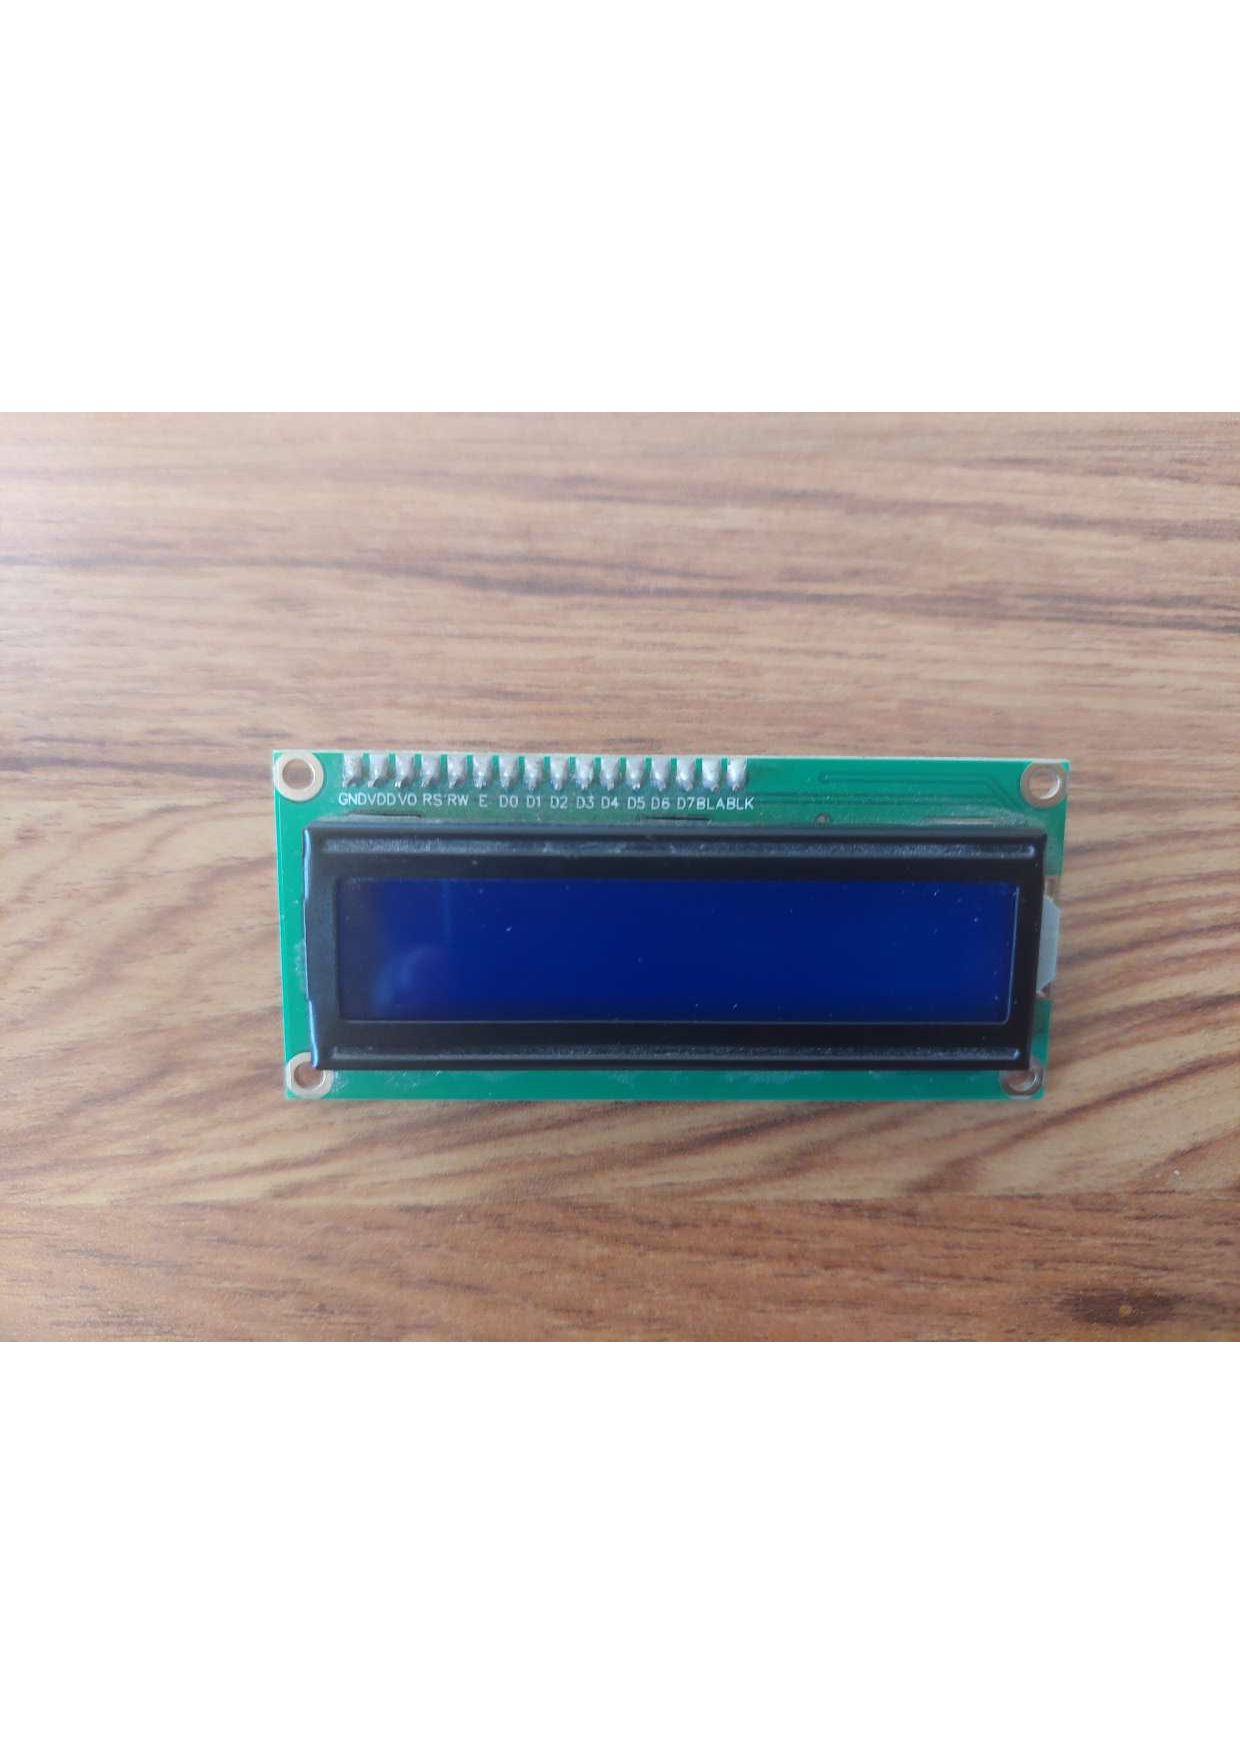
\includegraphics[trim = {0mm 0mm 0mm 0mm},clip,scale=0.2]{10/Img/lcd.pdf}
        \caption{LCD}
        \label{lcd}
\end{figure}

\textbf{Modulo adaptador}

El módulo I2C Interfaz LCD 16x2 es una solución popular para facilitar la conexión y el control de pantallas LCD con microcontroladores, reduciendo significativamente la cantidad de pines necesarios.

\begin{figure}[H]
        \centering
        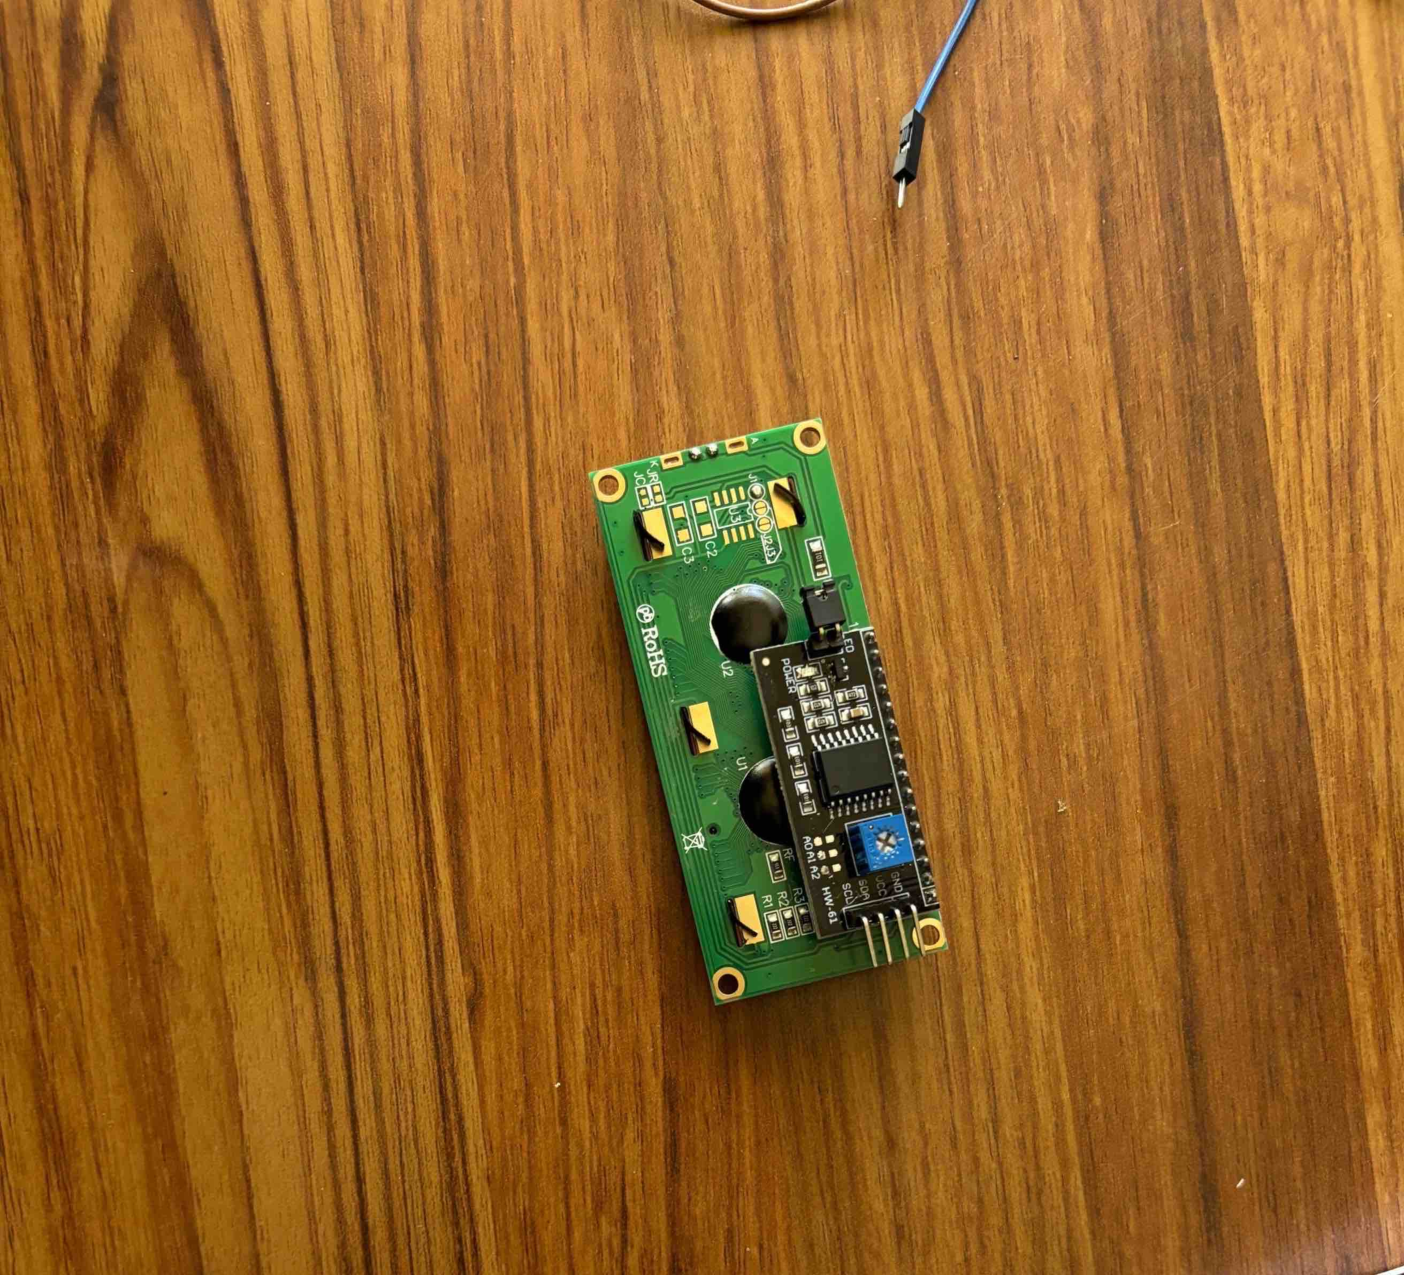
\includegraphics[trim = {30mm 30mm 30mm 30mm},clip,scale=0.2]{10/Img/moduloAdaptador.pdf}
        \caption{Modulo Adaptador}
        \label{Adaptador}
 \end{figure}

\textbf{ESP-32}

La ESP-32 es un potente microcontrolador de bajo costo y alto rendimiento, desarrollado por Espressif Systems, que incluye conectividad Wi-Fi y Bluetooth integrada. Es ampliamente utilizado en proyectos de Internet de las Cosas (IoT) debido a su versatilidad y capacidades avanzadas. 

\begin{figure}[H]
        \centering
        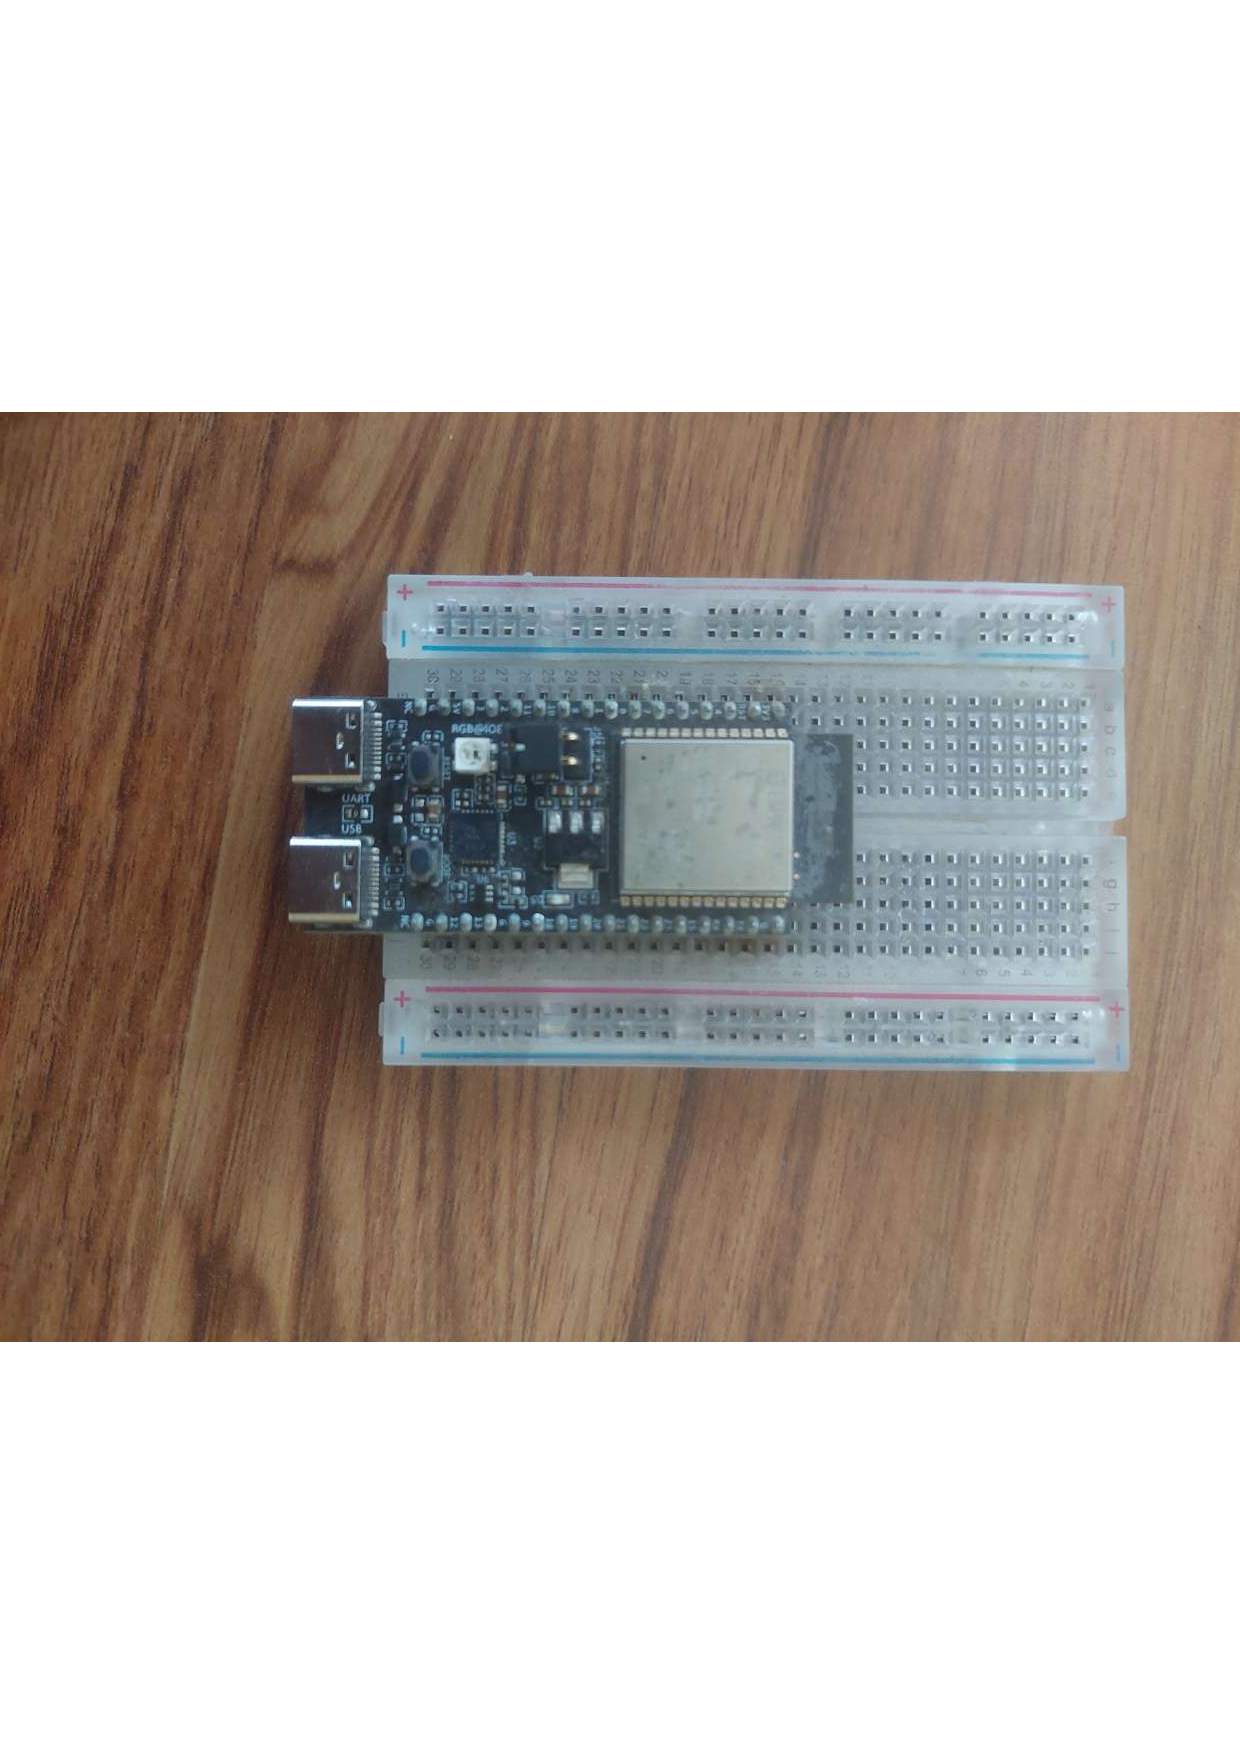
\includegraphics[trim = {40mm 120mm 50mm 100mm},clip,scale=0.2]{10/Img/esp-32.pdf}
        \caption{ESP-32}
        \label{ESP-32}
\end{figure}

\textbf{Potenciómetro}

Un potenciómetro es un dispositivo eléctrico de tres terminales que actúa como un divisor de voltaje ajustable. Es comúnmente utilizado para ajustar niveles de señal, calibrar dispositivos, y controlar volúmenes o niveles de brillo.
El potenciómetro funciona dividiendo la resistencia total entre las secciones a cada lado del wiper. Al ajustar el wiper, se cambia la proporción de la resistencia total entre los dos segmentos, lo que a su vez cambia el voltaje en el terminal central. \cite{Potenciómetro}

\begin{figure}[H]
        \centering
        \includegraphics[trim = {30mm 30mm 30mm 30mm},clip,scale=0.2]{10/Img/potenciómetro.pdf}
        \caption{Potenciómetro}
        \label{Potenciómetro}
\end{figure}

\textbf{Resistencia}

Una resistencia es un componente electrónico pasivo que limita el flujo de corriente eléctrica en un circuito. Es uno de los elementos básicos más utilizados en la electrónica.
La Resistencia Eléctrica es la oposición o dificultad al paso de la corriente eléctrica. Cuanto más se opone un elemento de un circuito a que pase por el la corriente, más resistencia va a tener. La resistencia eléctrica se mide en Ohmios y se representa con la letra R. Da igual emplear un símbolo u otro.\cite{Resistencias}

\begin{figure}[H]
        \centering
        \includegraphics[trim = {0mm 0mm 0mm 0mm},clip,scale=0.2]{10/Img/resistencias.pdf}
        \caption{Resistencias}
        \label{Resistencias}
\end{figure}

\textbf{Cables Dupont}

Los cables Dupont son cables de conexión flexibles que se utilizan comúnmente en prototipos de circuitos electrónicos y proyectos de desarrollo. Son conocidos por su facilidad de uso y versatilidad.
Se conoce así a los cables o alambres de calibre delgado con conectores tipo dupont en sus extremos, diseñados para conectarse en la mayoría de conectores tipo header o tiras de pines estándar de 0.1 pulgadas o 2.54 mm de espaciado.
Se utilizan principalmente como cables puente en protoboards y para interconectar tarjetas de desarrollo con sensores, módulos, actuadores, motores, etc. Suelen verse mucho en proyectos con Arduino o Raspberry Pi y son un material que se ha vuelto indispensable para estudiantes que trabajan con circuitos electrónicos.\cite{CablesDupont}

 \begin{figure}[H]
        \centering
        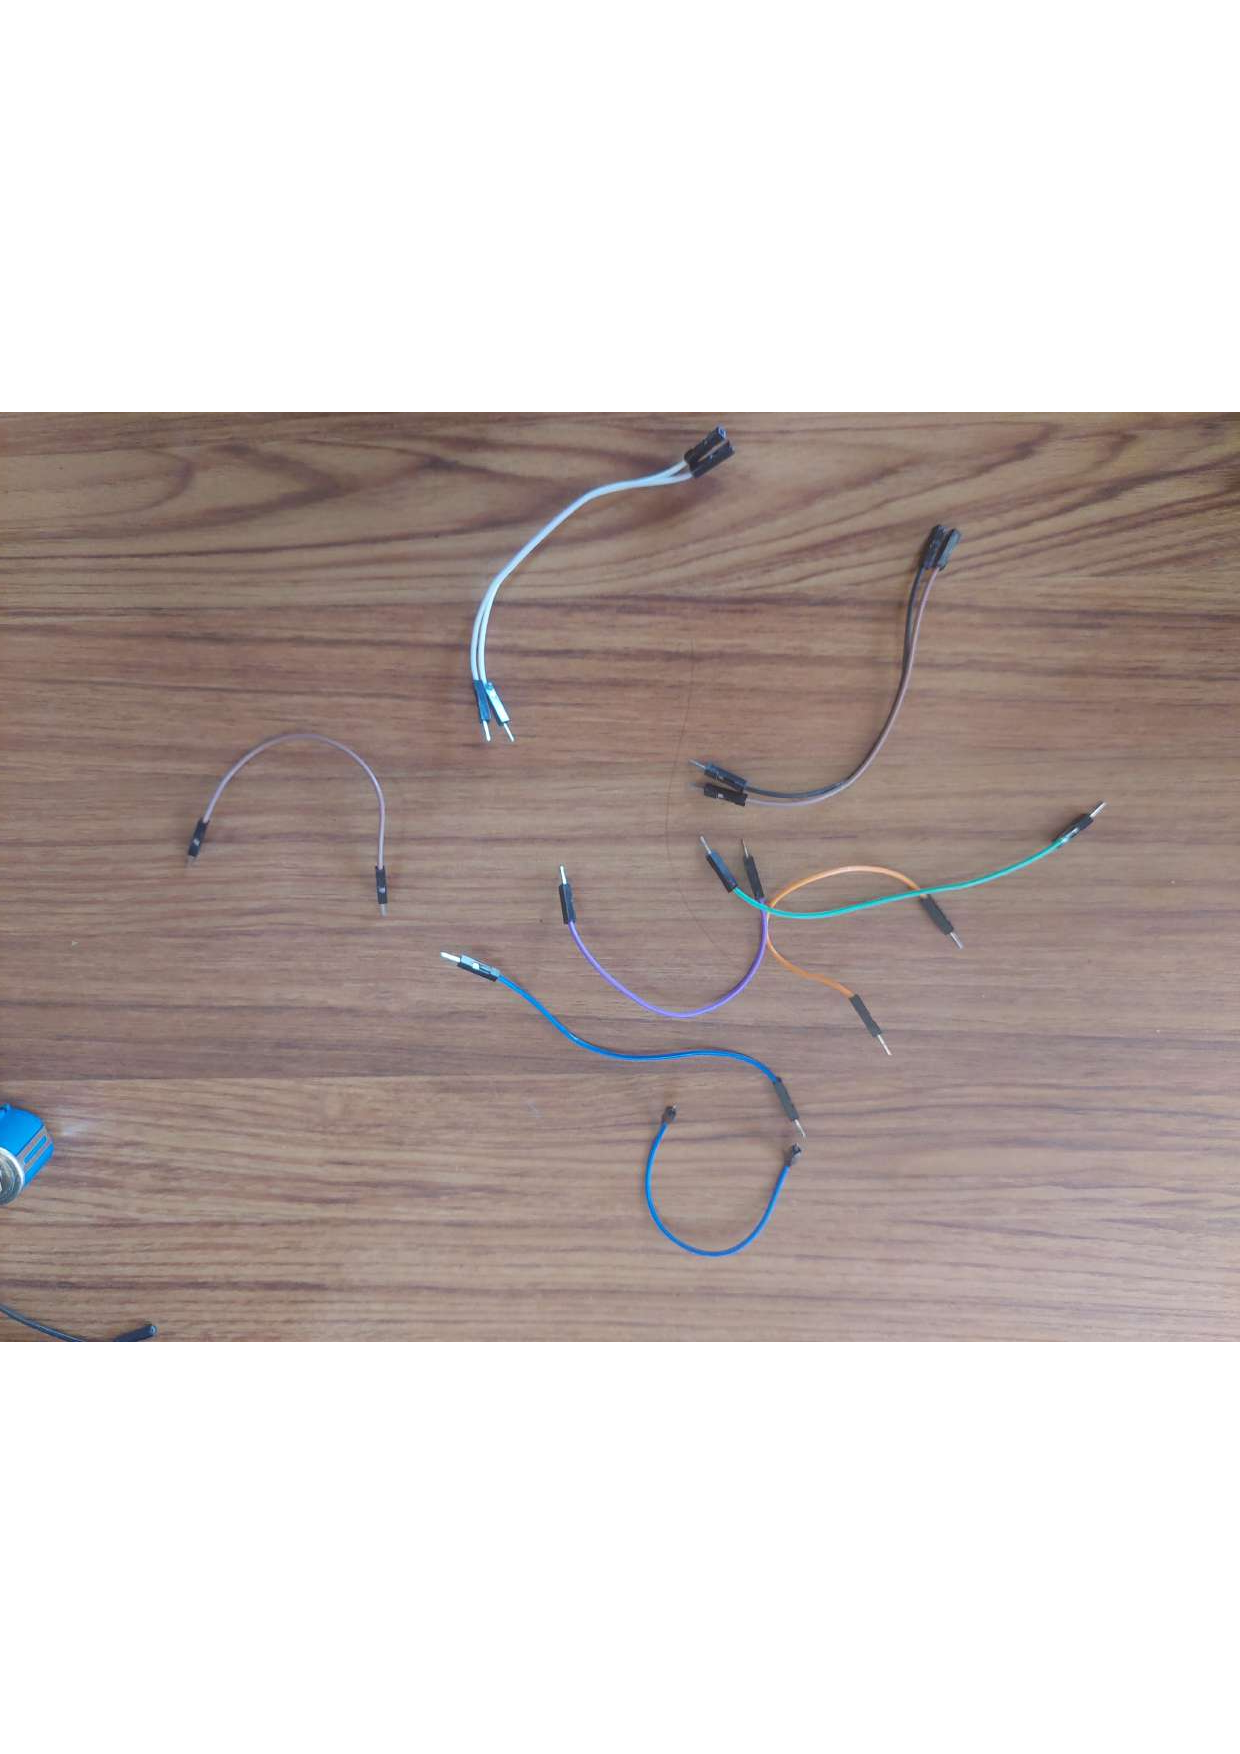
\includegraphics[trim = {30mm 30mm 30mm 30mm},clip,scale=0.2]{10/Img/cablesDupont.pdf}
        \caption{Cables Dupont}
        \label{Cables Dupont}
\end{figure}

\textbf{Regulador Multicontacto}

Un regulador multicontacto, también conocido como regulador de voltaje o estabilizador de tensión con múltiples salidas, es un dispositivo eléctrico diseñado para proporcionar un voltaje constante y estable a varios dispositivos conectados simultáneamente. Estos dispositivos son esenciales en entornos donde la calidad de la energía es crítica, y se utilizan para proteger equipos electrónicos sensibles de fluctuaciones de voltaje que pueden causar daños o mal funcionamiento.

 \begin{figure}[H]
        \centering
        \includegraphics[trim = {30mm 30mm 30mm 30mm},clip,scale=0.05]{10/Img/multicontacto.pdf}
        \caption{Multicontacto}
        \label{Multicontacto}
\end{figure}

\textbf{Cable tipo C}

Un cable tipo C, también conocido como USB-C, es un estándar de conexión de cables y conectores desarrollado para ser más versátil que sus predecesores. Su diseño permite una conexión reversible, lo que significa que no importa cuál sea la orientación del conector, siempre se puede insertar correctamente en el puerto. Además, el cable tipo C puede transportar datos, energía y señales de video, lo que lo hace muy versátil para una amplia gama de dispositivos, desde teléfonos inteligentes hasta computadoras portátiles y periféricos. Es un estándar cada vez más común en la industria electrónica debido a su capacidad para simplificar la conectividad y la carga de dispositivos.

\begin{figure}[H]
        \centering
        \includegraphics[trim = {90mm 45mm 90mm 80mm},clip,scale=0.05]{10/Img/cableUsb.pdf}
        \caption{Cable Usb}
        \label{Cable usb}
    \end{figure}
    
A continuación se presentan los dibujos de las
piezas que se utilizaron en el ensamble, en cada dibujo se muestra las medidas de cada una de las figuras:

\begin{figure}[H]
    \centering
    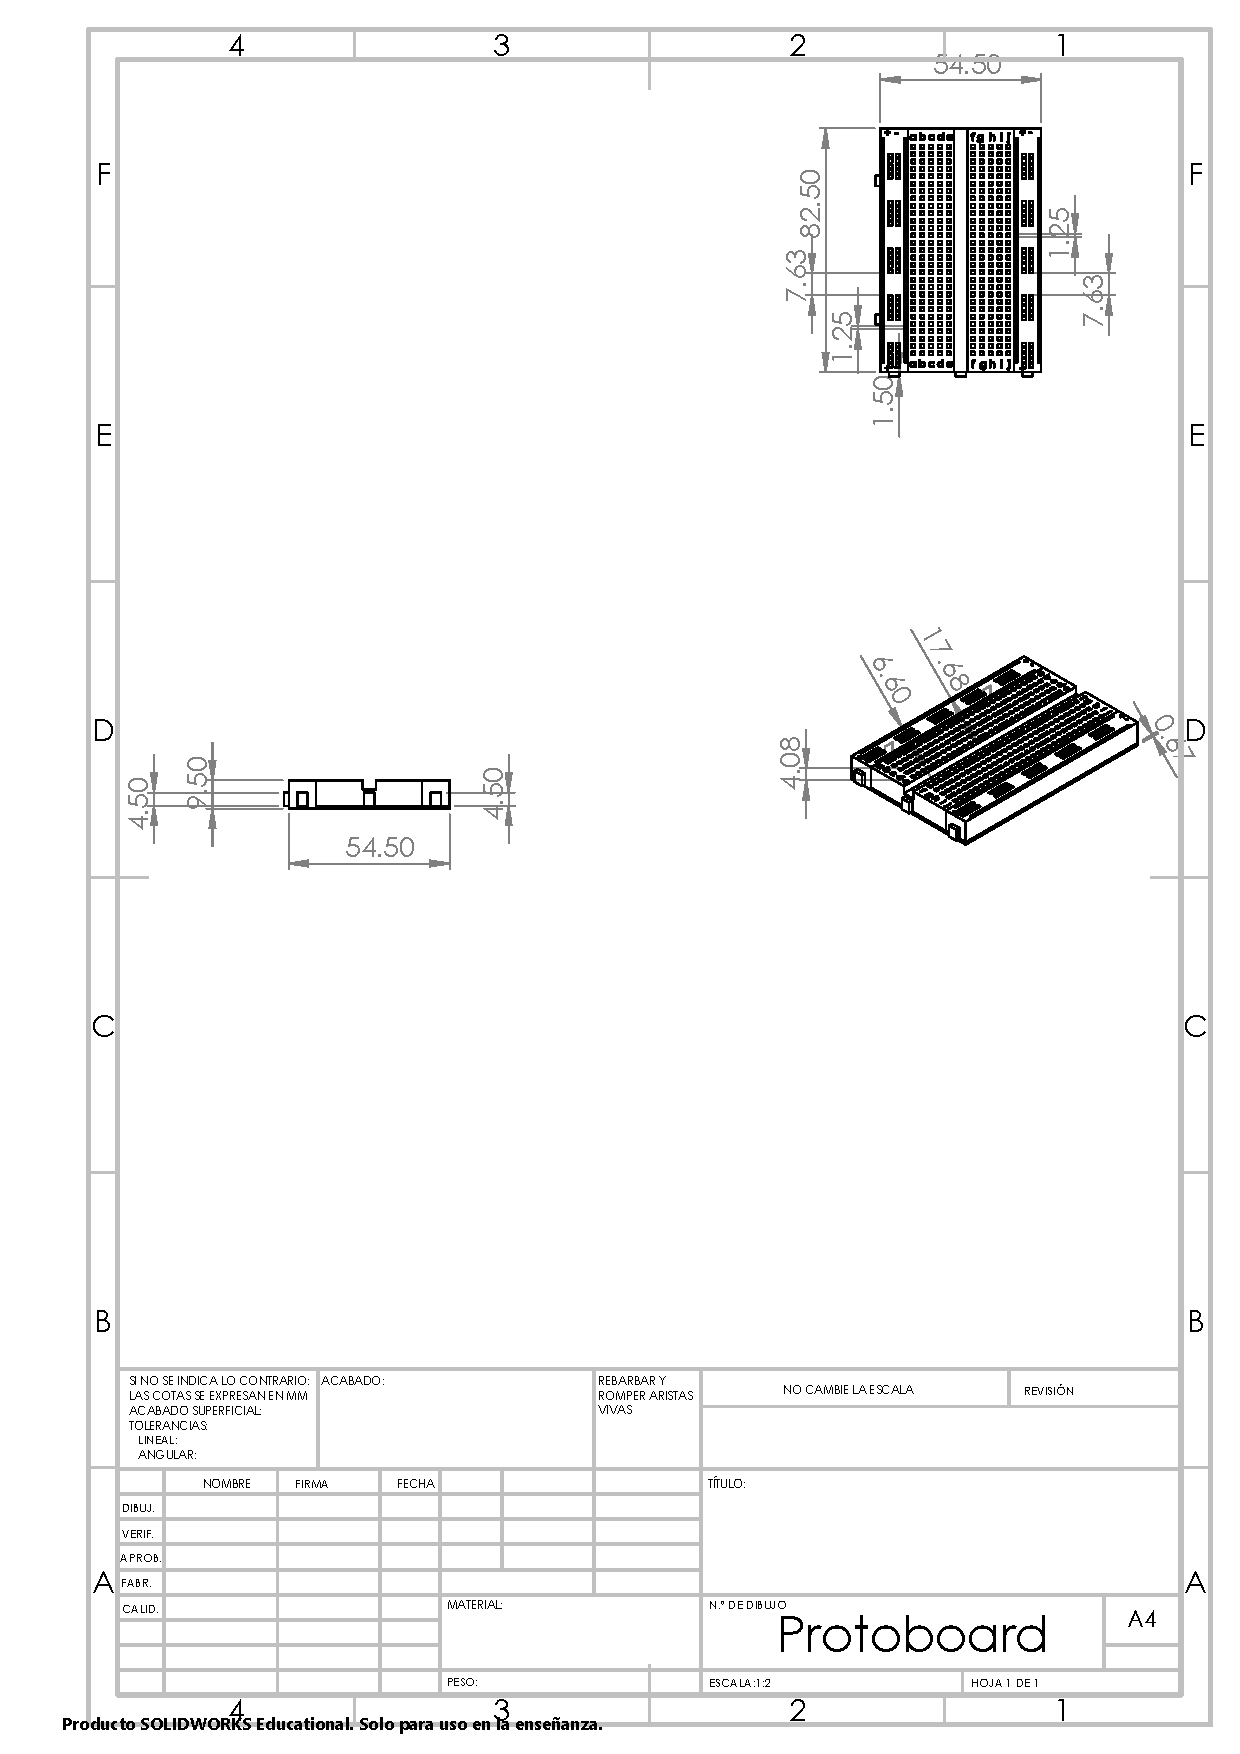
\includegraphics[scale=0.4]{10/Img/cotasProtoboard.pdf}
    \caption{Dibujo Protoboard}
    \label{fig:cotasProtoboard.png}
\end{figure}

\begin{figure}[H]
    \centering
    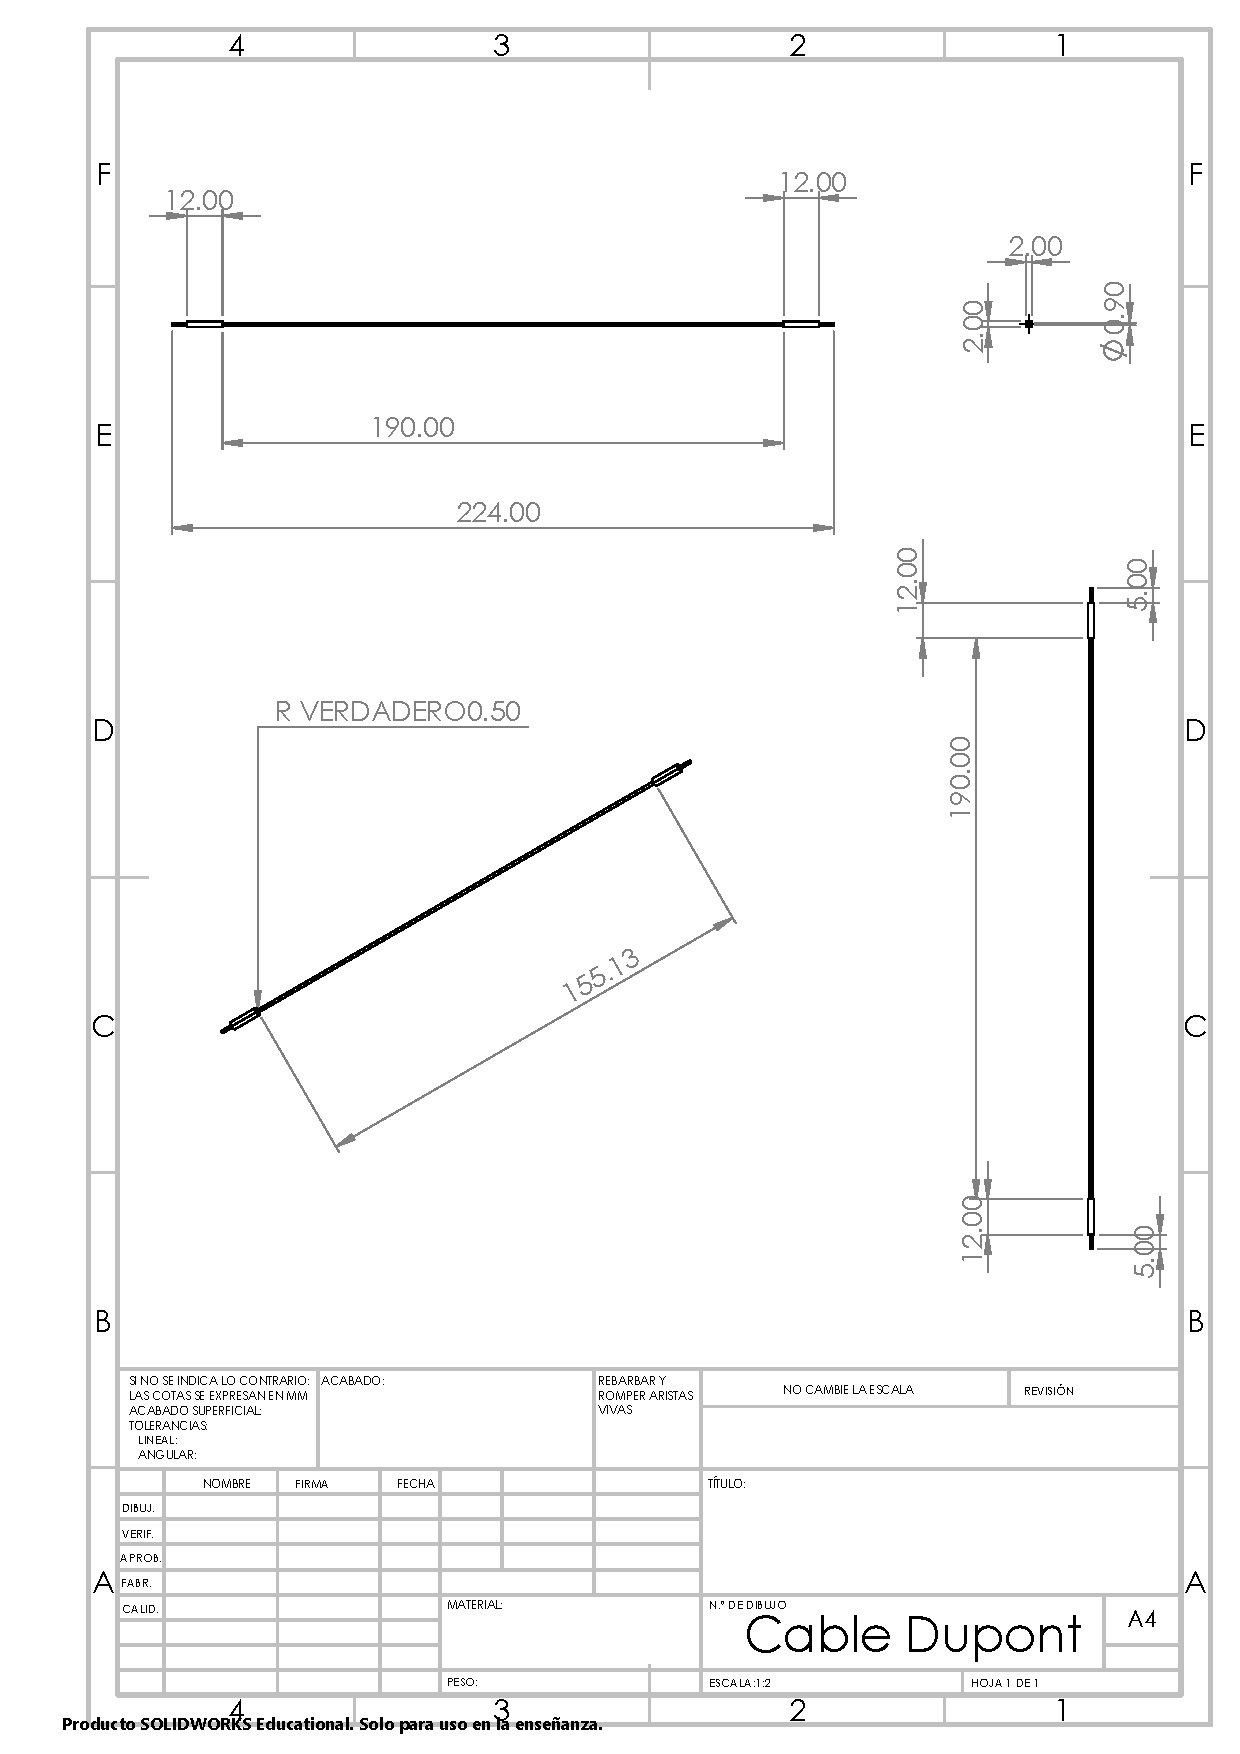
\includegraphics[scale=0.4]{10/Img/cotasDupont.pdf}
    \caption{Dibujo Cables Dupont}
    \label{fig:cotasdupont.png}
\end{figure}

\begin{figure}[H]
    \centering
    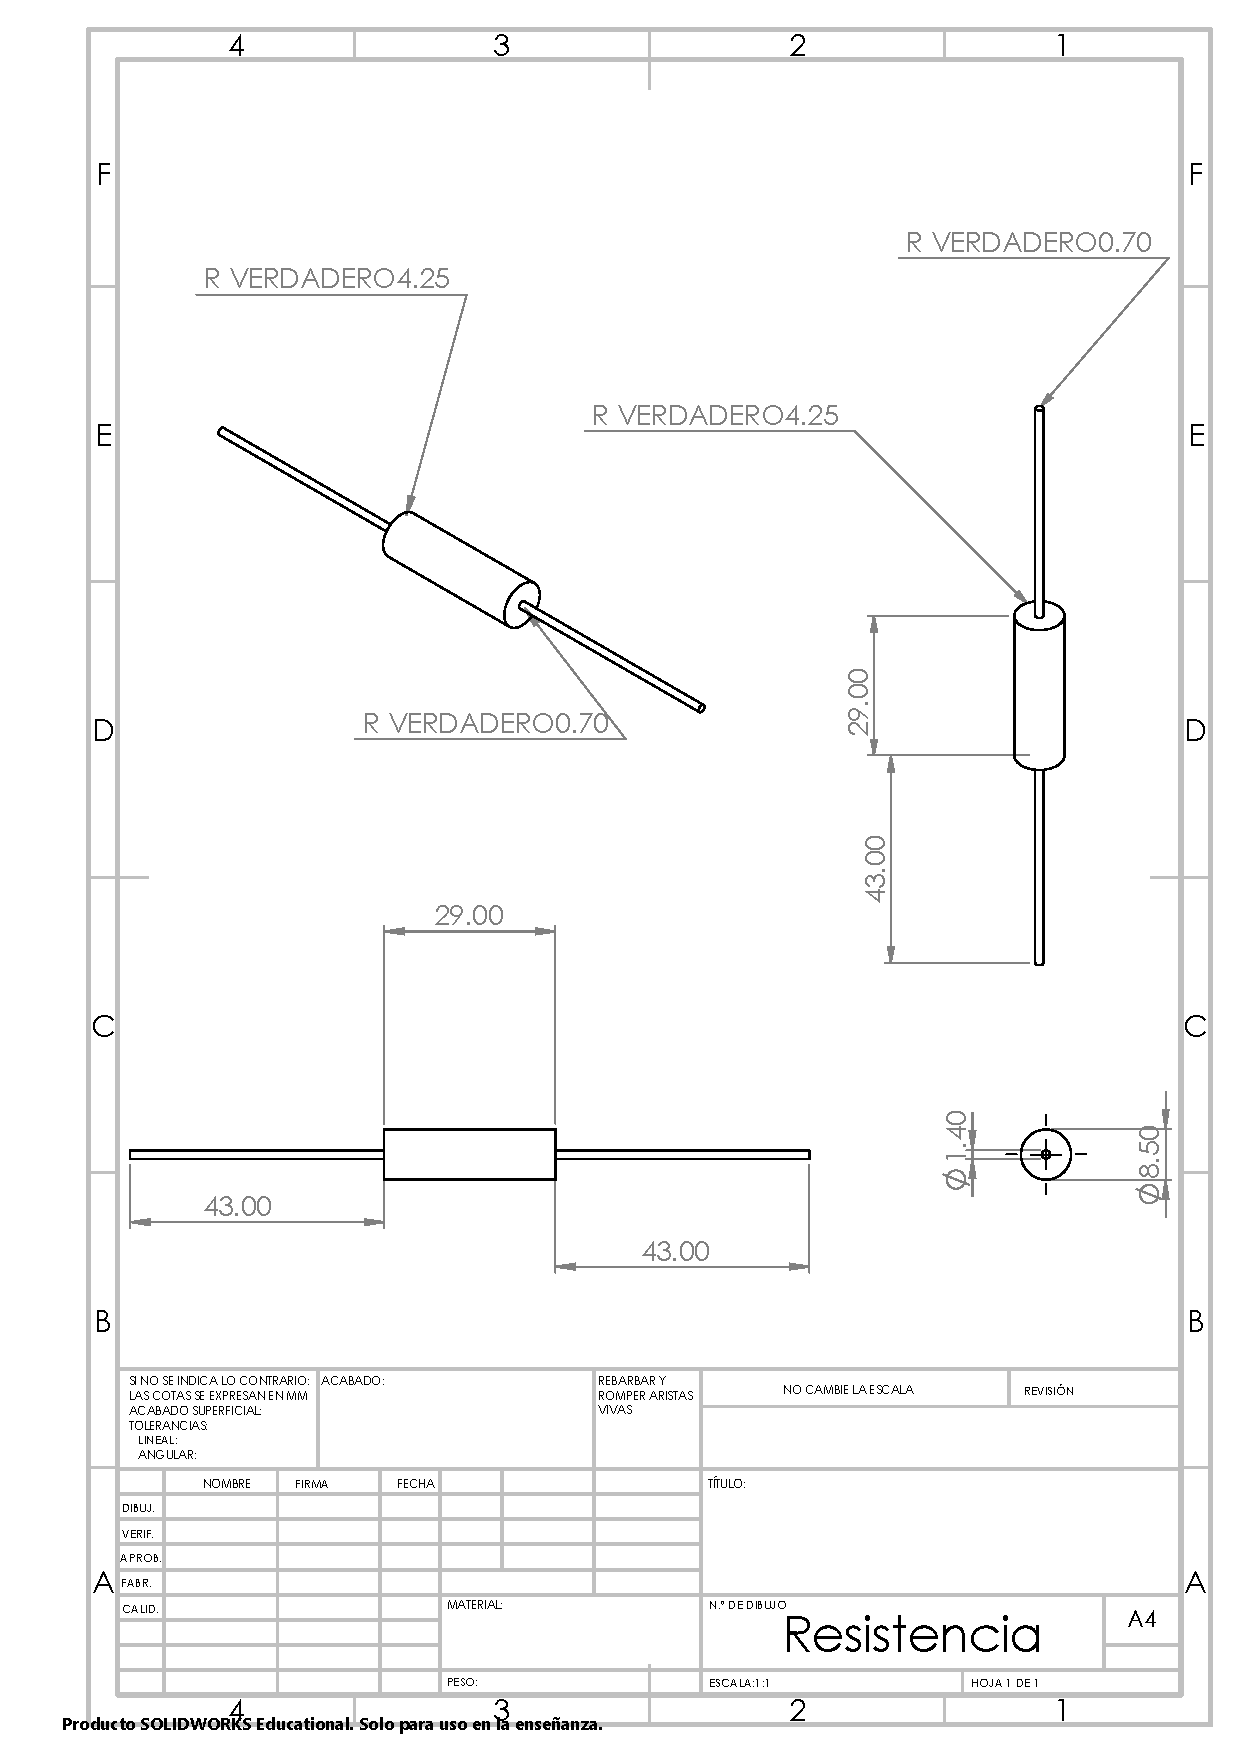
\includegraphics[scale=0.4]{10/Img/cotasResistencia.pdf}
    \caption{Dibujo Resistencia}
    \label{fig:cotasResistencia.png}
\end{figure}

\begin{figure}[H]
    \centering
    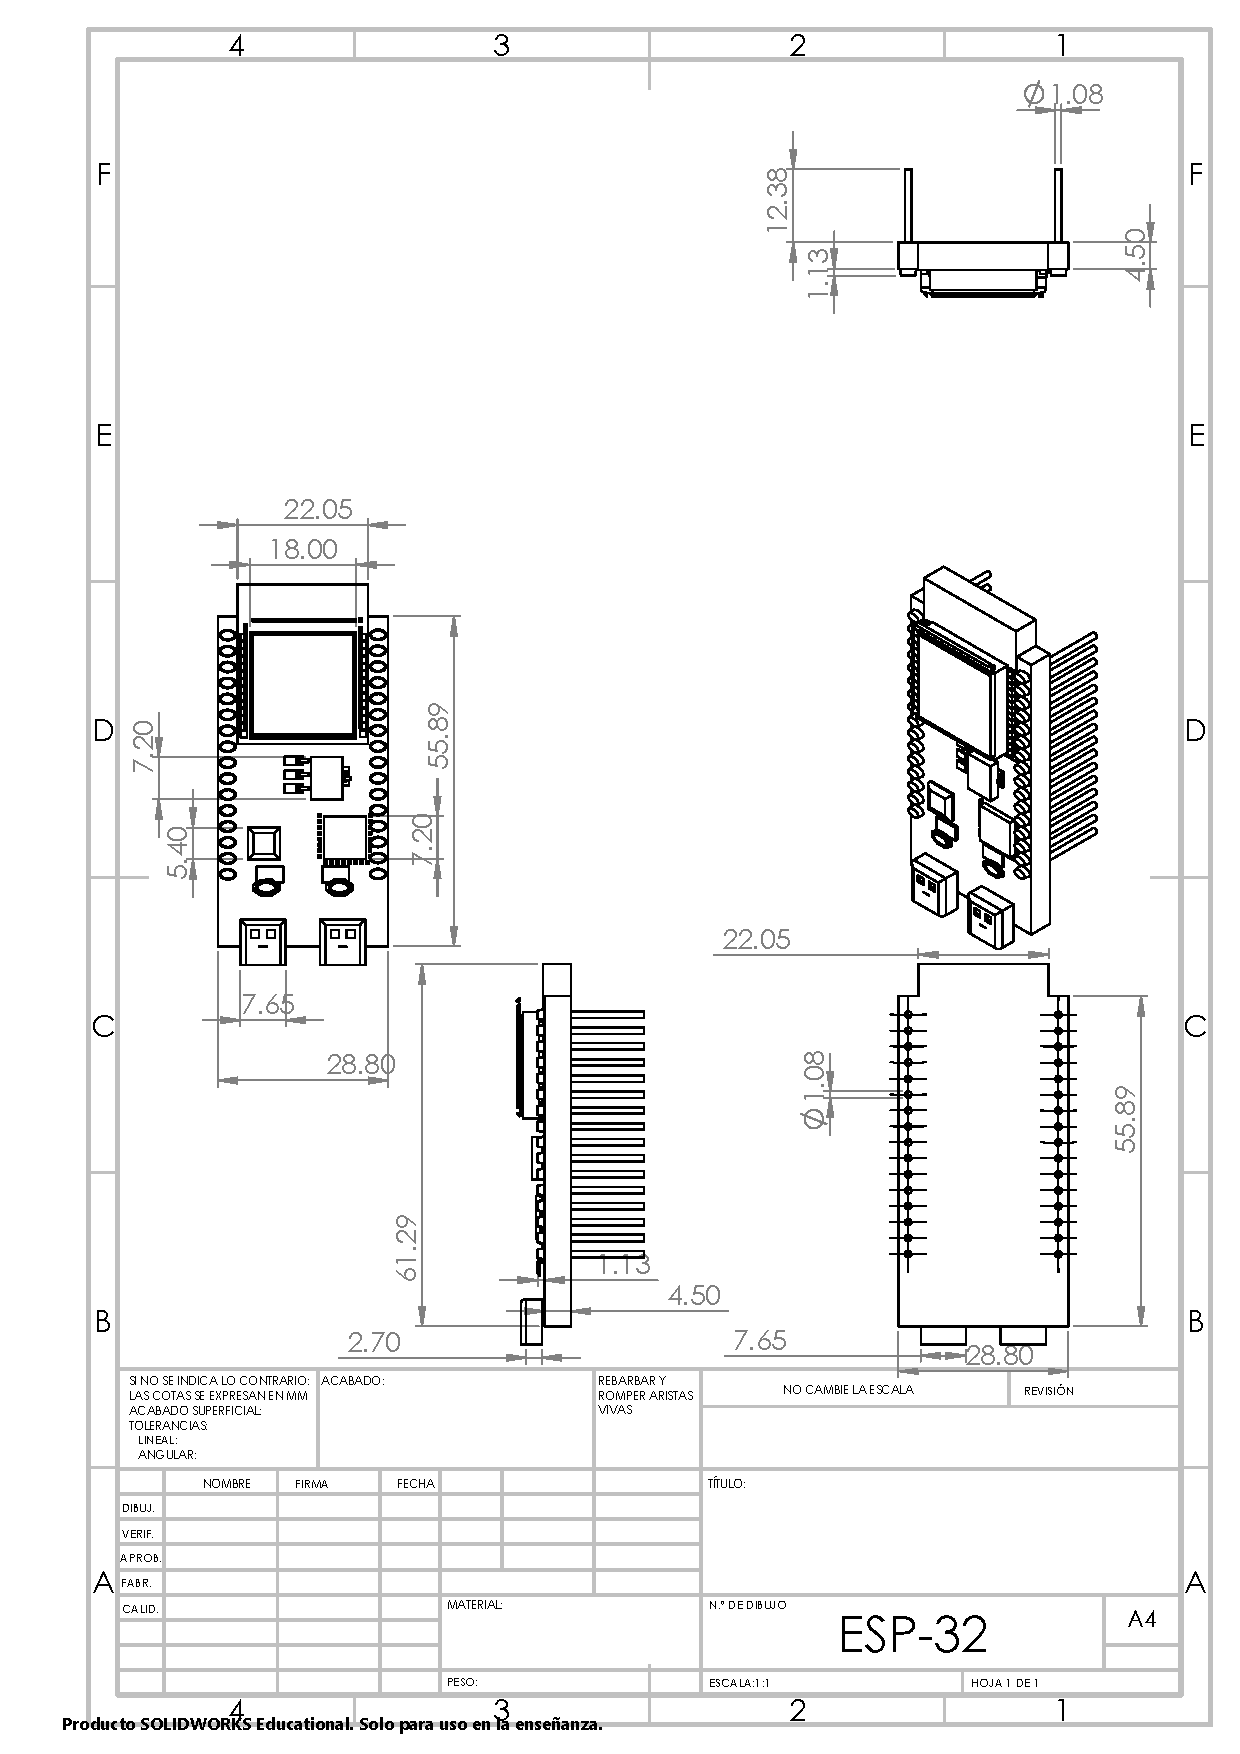
\includegraphics[scale=0.4]{10/Img/cotasEsp-32.pdf}
    \caption{Dibujo ESP-32}
    \label{fig:cotasEsp-32.png}
\end{figure}

\begin{figure}[H]
    \centering
    \includegraphics[scale=0.4]{10/Img/cotasPotenciómetro.pdf}
    \caption{Dibujo Potenciómetro}
    \label{fig:cotasPotenciómetro.png}
\end{figure}
%
%
\subsection{Determinación del tiempo estándar para que una persona competente realice el trabajo con marcha normal}

Para este momento ya se habrán obtenido el tiempo estándar en base a las muestras obtenidas y de esta manera con el método y los materiales también ya estandarizados se podrá llegar a un valor exacto de tiempo en el que se debe de realizar el trabajo.
%
%
% \subsection{Acrónimos y Abreviaciones}

% Los acrónimos y abreviaciones deberán ser definidos únicamente la primera vez que aparecen en el texto, esto para que el lector entienda lo que significan.

% \subsection{Ecuaciones}

% Las ecuaciones son una excepción a las especificaciones prescritas de esta plantilla. 
% Deberá determinar si su ecuación debe escribirse o no utilizando la fuente Adobe Devangari. 
% Para crear ecuaciones multinivel, puede ser necesario tratar la ecuación como un gráfico e insertarla en el texto después de aplicar el estilo de la platilla.
% Las ecuaciones serán enumeradas de manera consecutiva, y el número de ecuación, entre paréntesis, se colocan al ras de la derecha, utilizando una tabulación derecha.
% 
% \begin{equation}
%     \label{eq1}
%     x + y = z 
% \end{equation}
% 
% Es importante asegurarse de que los símbolos de la ecuación sean definidos antes o inmediatamente después de la ecuación. Utilice “(1)”, en vez de “Eq. 1” al enumerar las ecuaciones, excepto al principio de una oración: “La ecuación (\ref{eq1}) es…”

\section{Resultados y discusión}

\subsection{Desarrollo de la guía de plan de Emergencia}

Esta guía tiene como objetivo eliminar completamente las emergencias relacionadas con incendios y reducir el riesgo de accidentes en el Instituto Tecnológico de Querétaro. Para lograrlo, se identificará al personal que ha recibido capacitación al menos una vez al año, asegurando que, en caso de emergencia, puedan tomar las mejores decisiones para proteger la integridad física de todos, tanto dentro como fuera de la institución, y salvaguardar las instalaciones.
El objetivo del proyecto es realizar un análisis exhaustivo de los tiempos y movimientos involucrados en el ensamble de circuitos electrónicos, con el fin de identificar áreas de ineficiencia y oportunidades de mejora. A través de este análisis, se buscará implementar métodos y técnicas de optimización que permitan reducir los tiempos de producción, minimizar los movimientos innecesarios de los operarios y mejorar la calidad del producto final.
%
%

\begin{itemize}
    \item\textbf{Nombre comercial:} Instituto Tecnológico de Querétaro (ITQ)
    \item\textbf{Domicilio:} Av. Tecnológico s/n esq. Gral. Mariano Escobedo. Colonia Centro Histórico C.P. 76000, Querétaro, Qro. Figura \ref{fig:plano.png}
    \item\textbf{Teléfonos:} (442) 227 44 00 Ext. 4423 
    \item\textbf{Actividad principal:} Su actividad principal es ofrecer programas académicos de nivel superior, incluyendo licenciaturas, ingenierías, maestrías y doctorados, orientados a la preparación de recursos humanos altamente calificados para satisfacer las necesidades del sector industrial y tecnológico.
    \item\textbf{Superficie del establecimiento:} 78,575 m2
\end{itemize}
%
%
\begin{figure}[H]
    \centering
    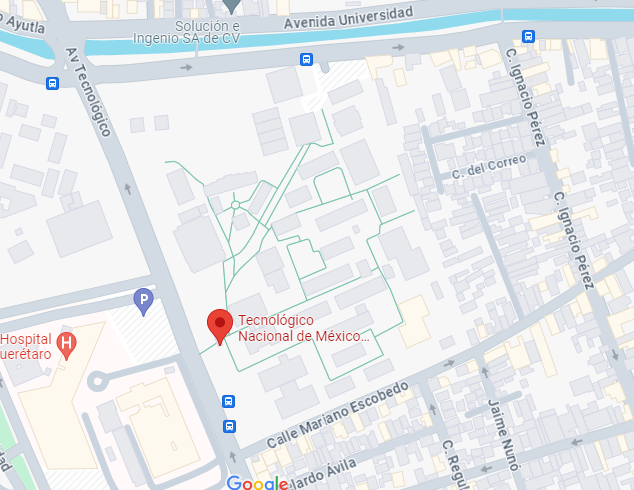
\includegraphics[scale=0.4]{10/Img/plano.png}
    \caption{Instituto Tecnológico de Querétaro}
    \label{fig:plano.png}
\end{figure}
%
%
\begin{figure}[H]
        \centering
        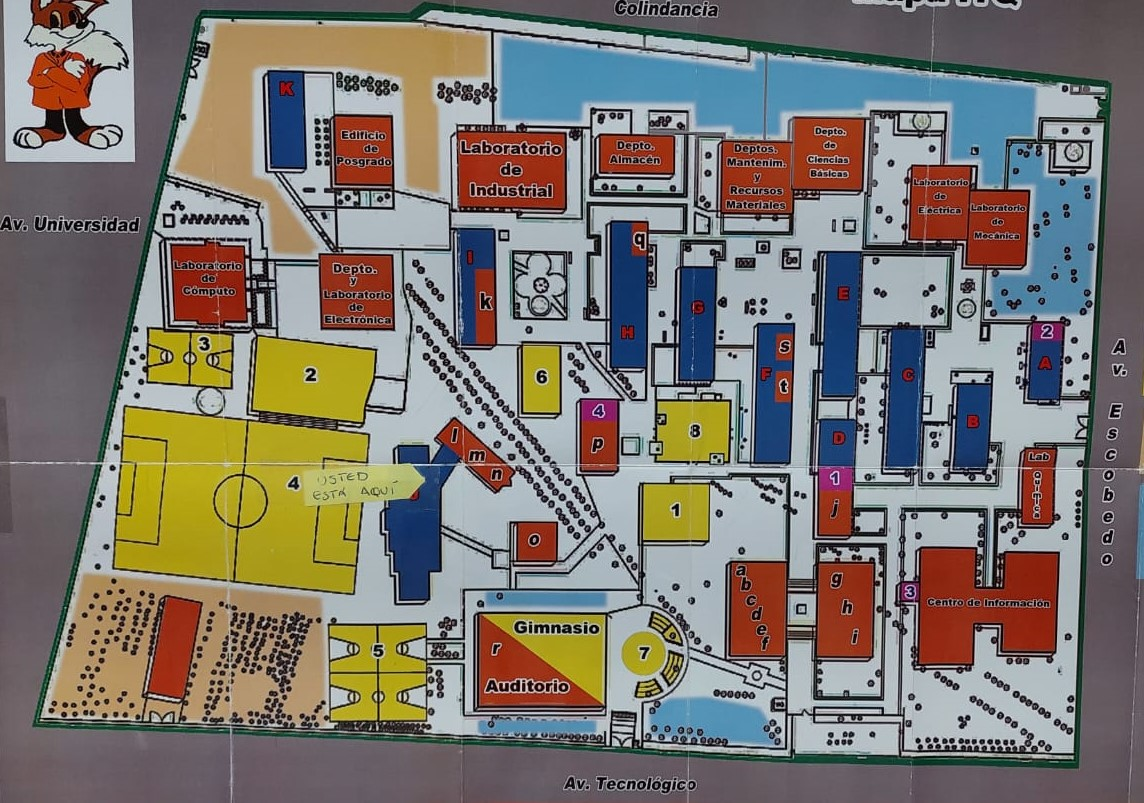
\includegraphics[trim = {0mm 0mm 0mm 0mm},clip,scale=0.2]{10/Img/mapa.jpg}
        \caption{Instituto Tecnológico de Querétaro. Av. Tecnológico s/n esq. Gral. Mariano Escobedo. Colonia Centro Histórico C.P. 76000, Querétaro, Qro.}
        \label{Mapa}
    \end{figure}
%
%
\subsubsection{Identificación del riesgo}

El riesgo se define como la combinación de la probabilidad de que se produzca un evento y sus consecuencias negativas. Los factores que lo componen son la amenaza y la vulnerabilidad.\cite{Riesgo}
\newline
El análisis de riesgos es un proceso fundamental para identificar, evaluar y priorizar los riesgos que pueden afectar a una organización, proyecto o cualquier otro ámbito en el que se desarrolle una actividad. Este proceso ayuda a tomar decisiones informadas para mitigar, transferir, aceptar o evitar dichos riesgos.

\begin{figure}[H]
    \centering
    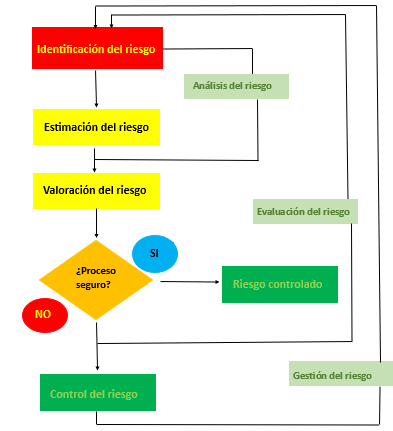
\includegraphics[scale=0.4]{10/Img/diagramaRiesgo.png}
    \caption{Diagrama Riesgos}
    \label{fig:diagramaRiesgo.png}
\end{figure}

\begin{table}[h]
        \centering
        \caption{Riesgos con diferentes niveles y colores para distinguir la gravedad y acciones}
        \begin{tabular}{c c c}
        \hline
        \multicolumn{3}{c}{\textbf{Riesgos}}\\
        \hline
             Alto& 0.99 - 0.18 & Rojo  \\
        \hline
             Medio& 0.17 - 0.05 & Amarillo  \\
        \hline
             Bajo& 0.04 - 0.01 & Verde \\
        \hline     
        \end{tabular}
        \label{tab:riego}
    \end{table}
%
%
\subsubsection{Riesgos Internos}

Los riesgos internos de una empresa son todos aquellos que dependen de nuestra gestión dentro de la Empresa y de los distintos departamentos que la componen. \cite{Riesgos}
%
%
\begin{figure}[H]
    \centering
    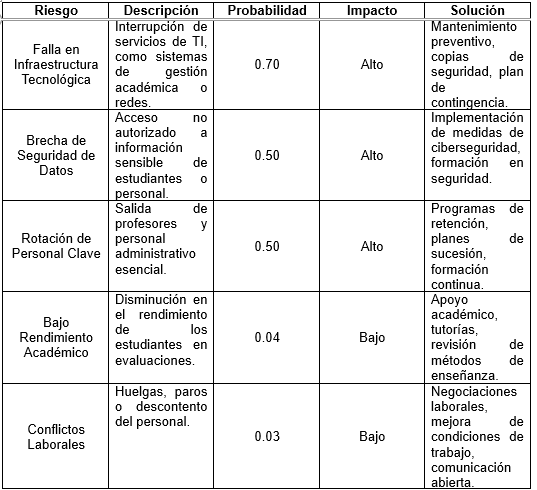
\includegraphics[scale=0.4]{10/Img/riesgosInternos.png}
    \caption{Riesgos Internos en una universidad}
    \label{fig:riesgosInternos.png}
\end{figure}
%
%
\subsubsection{Riesgos Externos}

Los riesgos externos de una empresa son todos aquellos que provienen del entorno de la Empresa y que influyen o condicionan su operativa pudiendo convertirse en amenazas para su desarrollo. \cite{Riesgos}
%
%
\begin{figure}[H]
    \centering
    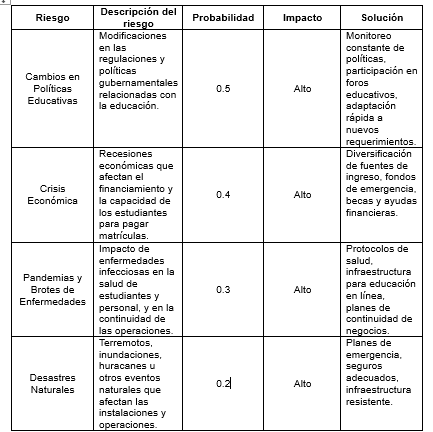
\includegraphics[scale=0.4]{10/Img/riesgosExternos.png}
    \caption{Riesgos Externos en una universidad}
    \label{fig:riesgosExternos.png}
\end{figure}
%
%
\subsubsection{Programa de actividades de prevención y auxilio}

El Instituto Tecnológico debe implementar medidas preventivas para proteger la salud de alumnos y trabajadores en caso de emergencias. Se proporcionó información sobre riesgos y se realizan simulacros semestrales para evacuar edificios y reunirse en puntos designados. Además, se presentó el área de atención médica cerca de los edificios J, que ofrece apoyo médico y psicológico. Sin embargo, un estudio reveló deficiencias en la sala médica, con un botiquín mínimo que solo contiene analgésicos básicos y material para heridas leves. Además, el tanque de gas y muchos extintores no están rellenados, indicando una falta de medidas de seguridad adecuadas en la mayoría de los edificios, excepto en el centro de información y laboratorios.
% 
% 
\subsubsection{Plan de acción}

Se debe elaborar un plan de acción para abordar los riesgos internos y externos identificados. Este plan debe incluir medidas preventivas para evitar que los riesgos se materialicen, instrucciones sobre qué hacer si ya ocurrieron, y un seguimiento de los resultados de estas acciones.

%
%
\subsubsection{Identificación de capacidades}

\begin{table}[H]
    \centering
    \caption{Recursos en materia de seguridad}
    \begin{tabular}{c c c}
    \hline
    \multicolumn{3}{c}{Inventario de recursos en materia de seguridad}\\
    \hline
         No.& Recurso & Cantidad  \\
    \hline
         1& Extintor & 39  \\
    \hline
         2& Botiquín & 0  \\
    \hline
         3& Detector de humo & 0 \\
    \hline
         4& Lampara de emergencia & 0 \\
    \hline     
    \end{tabular}
    \label{tab:inventario}
\end{table}
%
%
\subsubsection{Plano de localización de recursos}
%
%
\begin{figure}[H]
        \centering
        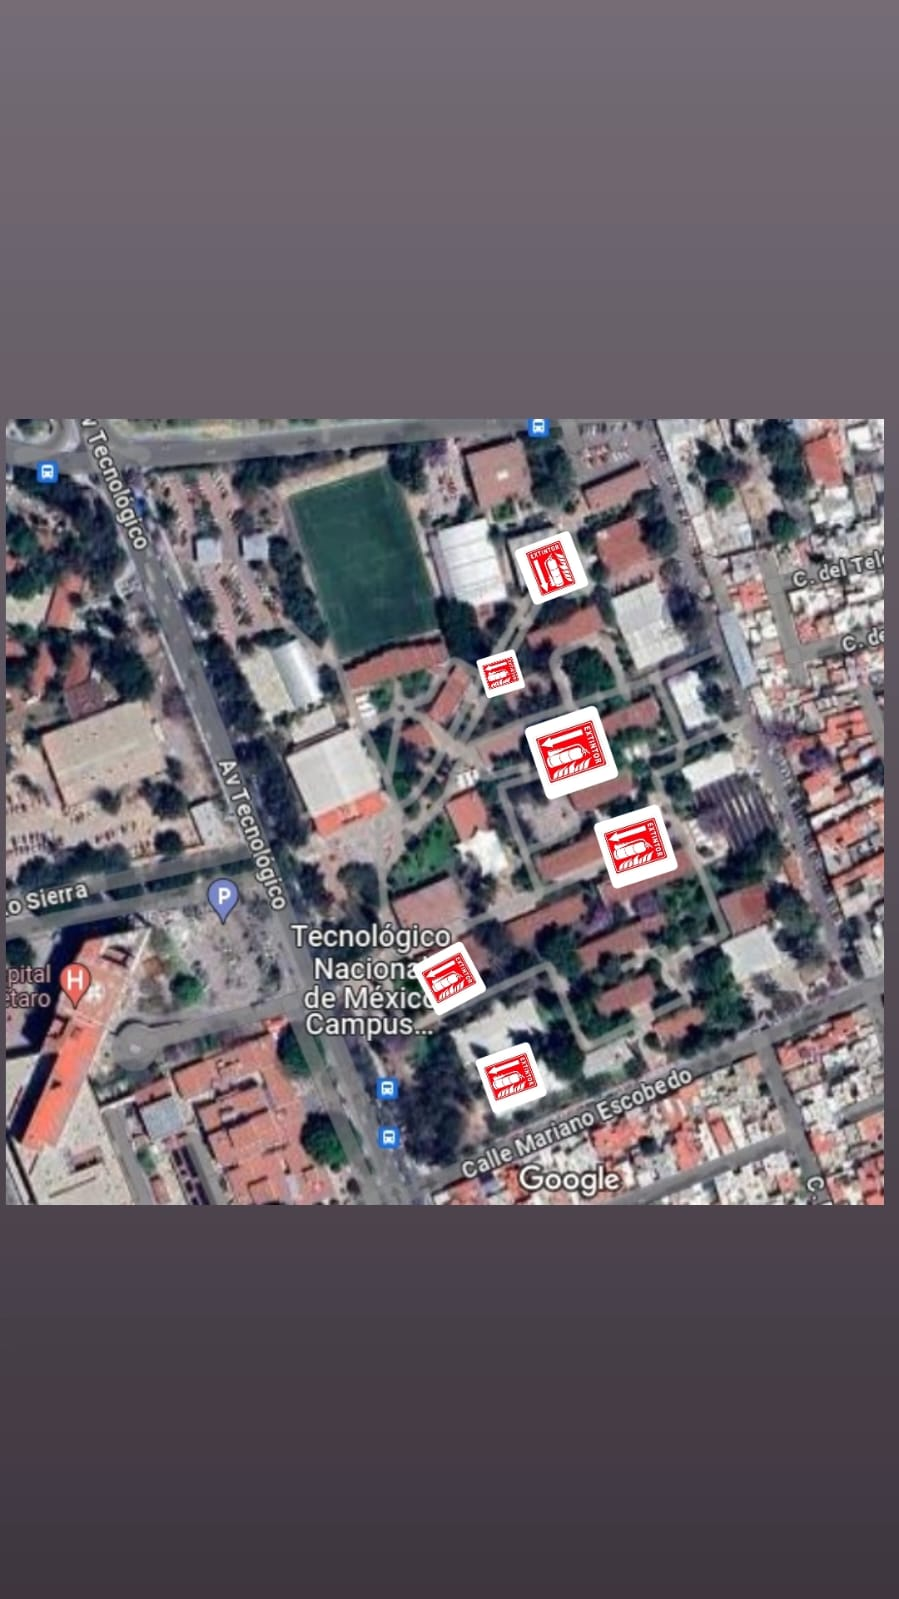
\includegraphics[trim = {30mm 120mm 30mm 120mm},clip,scale=0.2]{10/Img/recursos.jpg}
        \caption{Identificación de extintores}
        \label{Recursos}
    \end{figure}
%
%
\subsubsection{ Identificación de apoyos externos}

\begin{figure}[H]
    \centering
    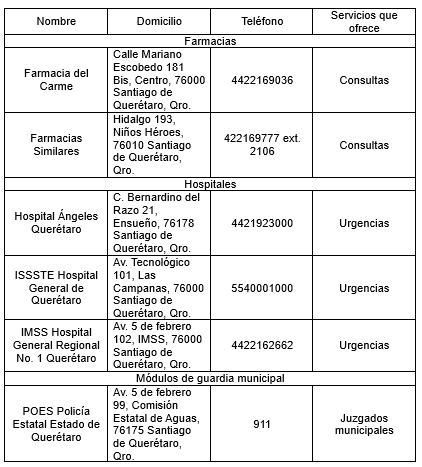
\includegraphics[scale=0.4]{10/Img/apoyos.png}
    \caption{Apoyos externos a la institución}
    \label{fig:apoyos.png}
\end{figure}
%
%
\subsubsection{Identificación de puntos de reunión}

\begin{figure}[H]
        \centering
        \includegraphics[trim = {0mm 0mm 0mm 0mm},clip,scale=0.2]{10/Img/puntoReunión.jpg}
        \caption{Puntos de Reunión}
        \label{Puntos de Reunión}
    \end{figure}
%
%
\subsubsection{Brigada de evacuación}

\begin{figure}[H]
    \centering
    \includegraphics[scale=0.4]{10/Img/brigadaEvacuación.png}
    \caption{Brigada de Evacuación}
    \label{fig:brigadaEvacuación.png}
\end{figure}
%
%
\subsubsection{Directorio de telefónicos de emergencia}

\begin{figure}[H]
    \centering
    
\includegraphics[scale=0.4]{10/Img/911.jpg}
    \caption{Números de emergencia }
    \label{fig:911.png}
\end{figure}

\begin{figure}[H]
    \centering
    \includegraphics[scale=0.4]{10/Img/númerosEmergencia.png}
    \caption{Números de emergencia más próximos a la institución }
    \label{fig:númerosEmergencia.png}
\end{figure}
% \begin{itemize}
       % \item Se debe establecer que se habrá de hacer, como, conque, y donde para obtener la información que permita probar la hipótesis.  
        %\item Se debe desglosar de acuerdo a los objetivos específicos. 
        %\item Se debe establecer una estrategia metodológica por cada objetivo específico. De manera simplista se podría decir que se cambia el verbo en infinitivo por su respectivo adverbio.
        %\item En cada objetivo se debe describir que método, que materiales y que equipo se usará para conseguirlo.
        %\item Se deben tener referencias Figura 
%  \end{itemize}
    % 
    % 
%\subsection{Prepara tu documento}
    
  %  Antes de que comiences a utilizar esta plantilla, es recomendable que prepare la información que contendrá en un archivo aparte. 
   % Ten preparadas tus gráficas, así como también las tablas aparte, para que sea más fácil integrarlo. 
    %Se recomienda fuertemente el uso de \textbf{formato Enhanced Metafile (.emf) para imágenes y gráficas} de resolución óptima. 
    %Finalmente, completa y organiza el contenido antes de darle el formato de esta plantilla. 
    
    %\subsection{Acrónimos y Abreviaciones}
    
   % Los acrónimos y abreviaciones deberán ser definidos únicamente la primera vez que aparecen en el texto, esto para que el lector entienda lo que significan.
    
    %\subsection{Ecuaciones}

%Una ecuación en matemática es una igualdad establecida entre dos expresiones, en la cual puede haber una o más incógnitas que deben ser resueltas.

%Las ecuaciones sirven para resolver diferentes problemas matemáticos, geométricos, químicos, físicos o de cualquier otra índole, que tienen aplicaciones tanto en la vida cotidiana como en la investigación y desarrollo de proyectos científicos.

%Las ecuaciones pueden tener una o más incógnitas, y también puede darse el caso de que no tengan ninguna solución o de que sea posible más de una solución. \cite{Ecuacion}

%Las ecuaciones son una excepción a las especificaciones prescritas de esta plantilla. 
%Deberá determinar si su ecuación debe escribirse o no utilizando la fuente Adobe Devangari. 
%Para crear ecuaciones multinivel, puede ser necesario tratar la ecuación como un gráfico e insertarla en el texto después de aplicar el estilo de la platilla.
%Las ecuaciones serán enumeradas de manera consecutiva, y el número de ecuación, entre paréntesis, se colocan al ras de la derecha, utilizando una tabulación derecha. 
    
%    \begin{equation}
%  \label{eq1}
%       x + y = z 
%        \end{equation}
    
%Es importante asegurarse de que los símbolos de la ecuación sean definidos antes o inmediatamente después de la ecuación. Utilice “(1)”, en vez de “Eq. 1” al enumerar las ecuaciones, excepto al principio de una oración: “La ecuación (\ref{eq1}) es…”


\subsection{Análisis de los métodos, materiales, herramientas e instalación utilizada en la ejecución del ensamble de un circuito electrónico}

\subsubsection{Verificación}

La planeación no salió como se esperaba, ya que durante el proceso de ensamblaje ocurrió un accidente y la ESP-32 se dañó, lo que provocó un retraso en el trabajo al contar solo con una unidad. Para solucionar este problema, decidimos comprar una nueva ESP-32, por lo que tuvimos que detener todo, ya que, el tiempo de espera para que llegara la nueva ESP fue de 2 semanas. Al darnos cuenta de este problema, tomamos una decisión drástica: que cada pareja comprara una ESP-32 o que cada quien de manera individual la comprara. Además de que una vez que la ESP-32 llegara debía ser programada por el profesor, lo que hizo que se perdiera aun más tiempo. Se realizó una serie de comparaciones en cuanto a costo, calidad y tiempo de llegada del producto. Finalmente, realizamos un pedido grande a través de una plataforma de compras en línea.La inversión final fue de 244 pesos por persona o por pareja.

\begin{figure}[H]
        \centering
        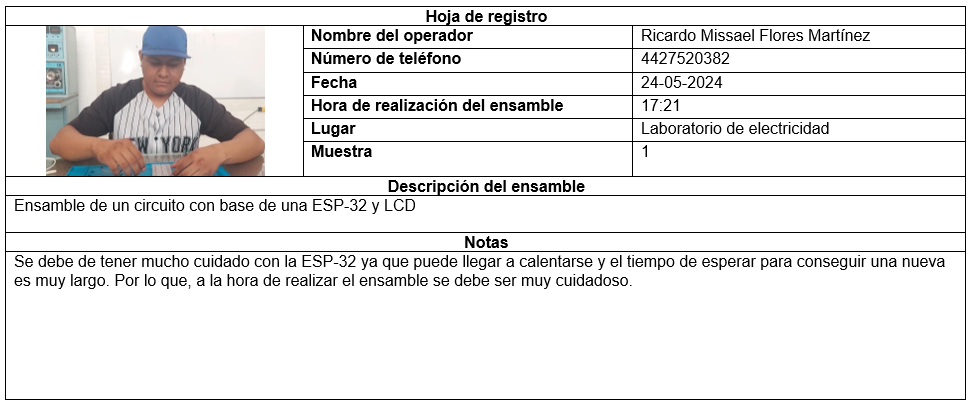
\includegraphics[trim = {0mm 0mm 0mm 0mm},clip,scale=0.2]{10/Img/hojaRegistro1.png}
        \caption{Hoja de registro de la primera muestra}
        \label{hojaRegistro1}
    \end{figure}

A continuación se muestran las evidencias de la primera muestra del ensamble:

\begin{figure}[H]
        \centering
        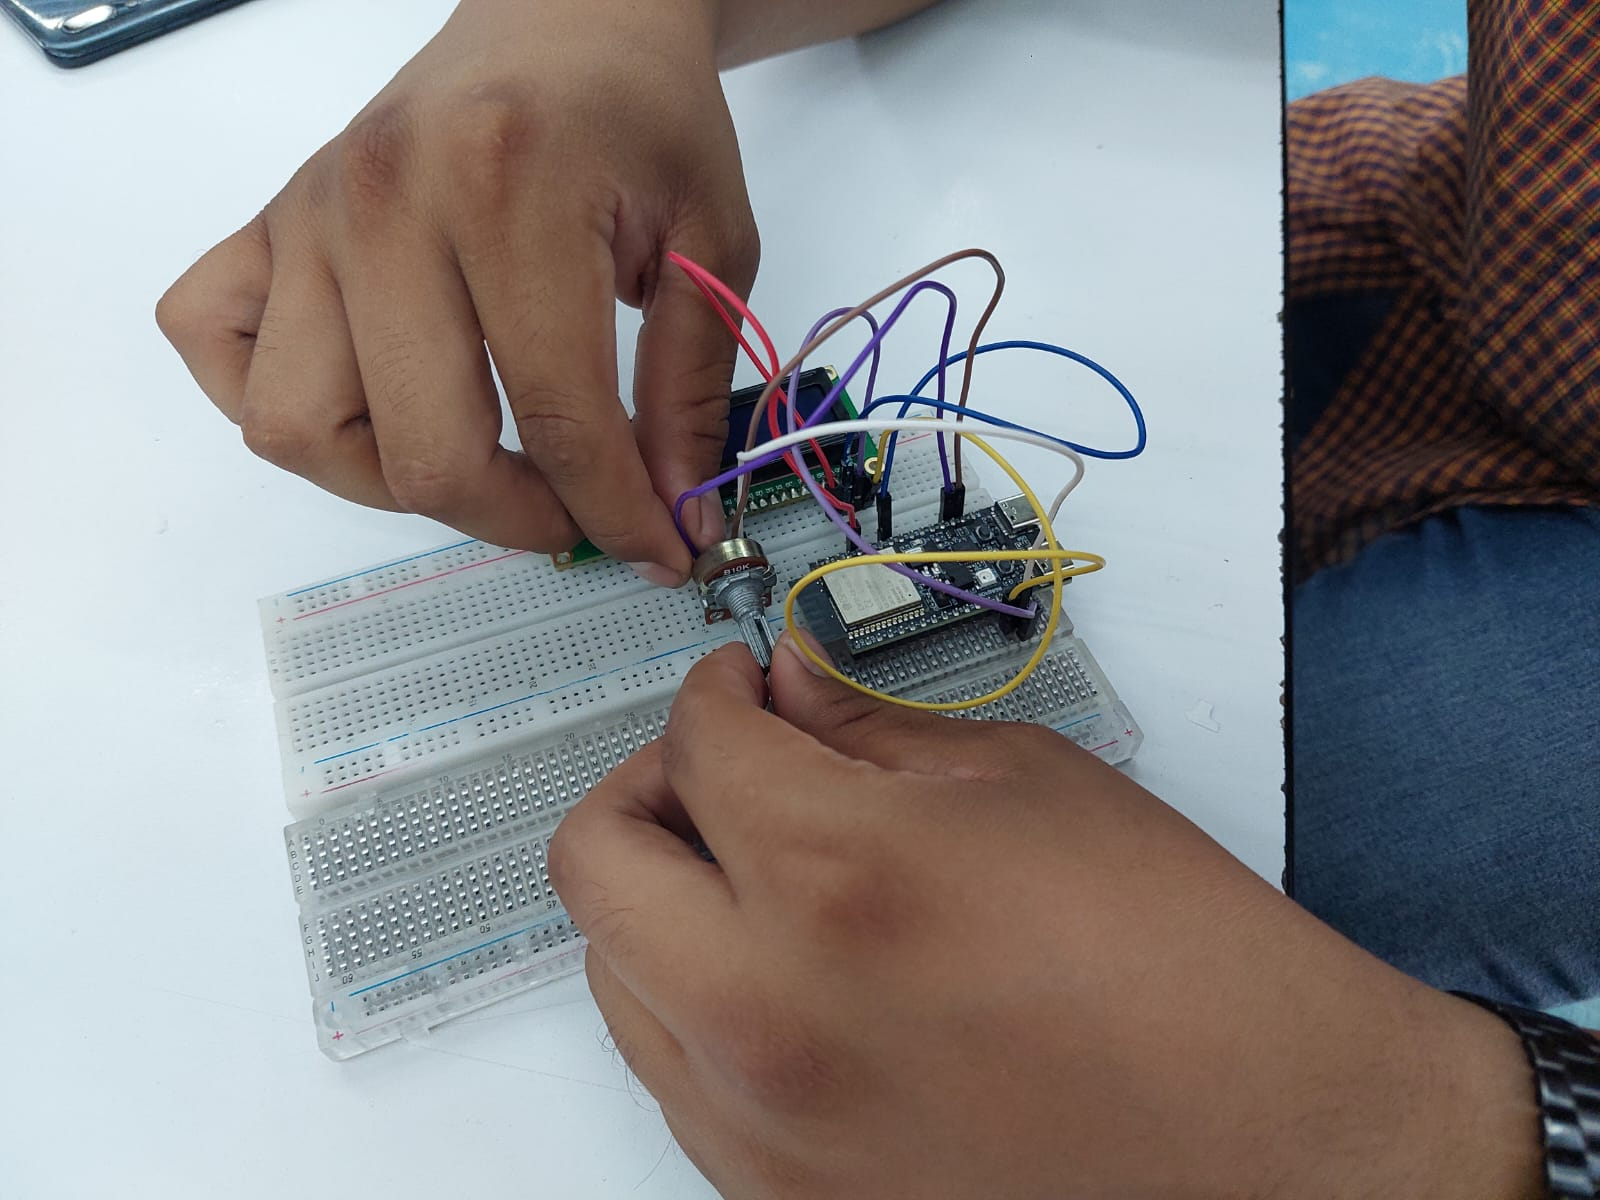
\includegraphics[trim = {0mm 0mm 0mm 0mm},clip,scale=0.2]{10/Img/muestra1Prueba1.jpg}
        \caption{Evidencia 1 de la primera muestra}
        \label{muestra1Prueba1}
    \end{figure}

\begin{figure}[H]
        \centering
        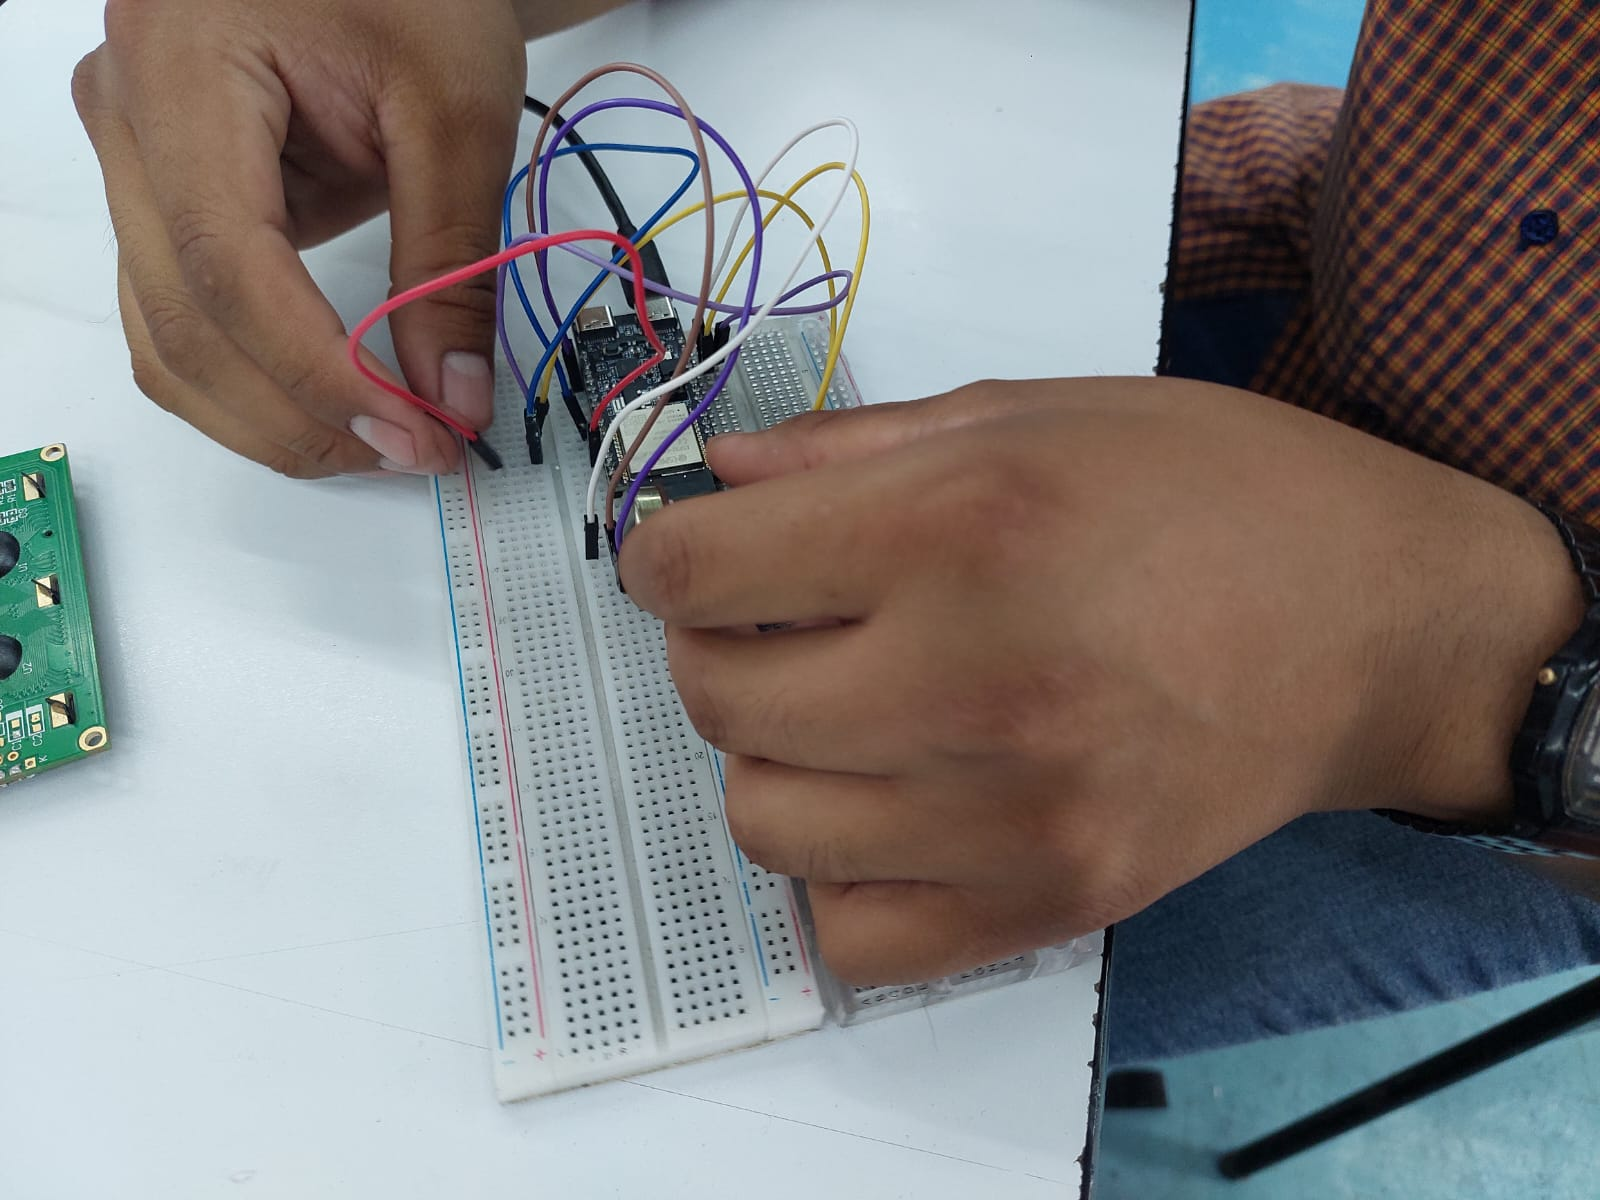
\includegraphics[trim = {0mm 0mm 0mm 0mm},clip,scale=0.2]{10/Img/muestra1Prueba2.jpg}
        \caption{Evidencia 2 de la primera muestra}
        \label{muestra1Prueba2}
    \end{figure}

\begin{figure}[H]
        \centering
        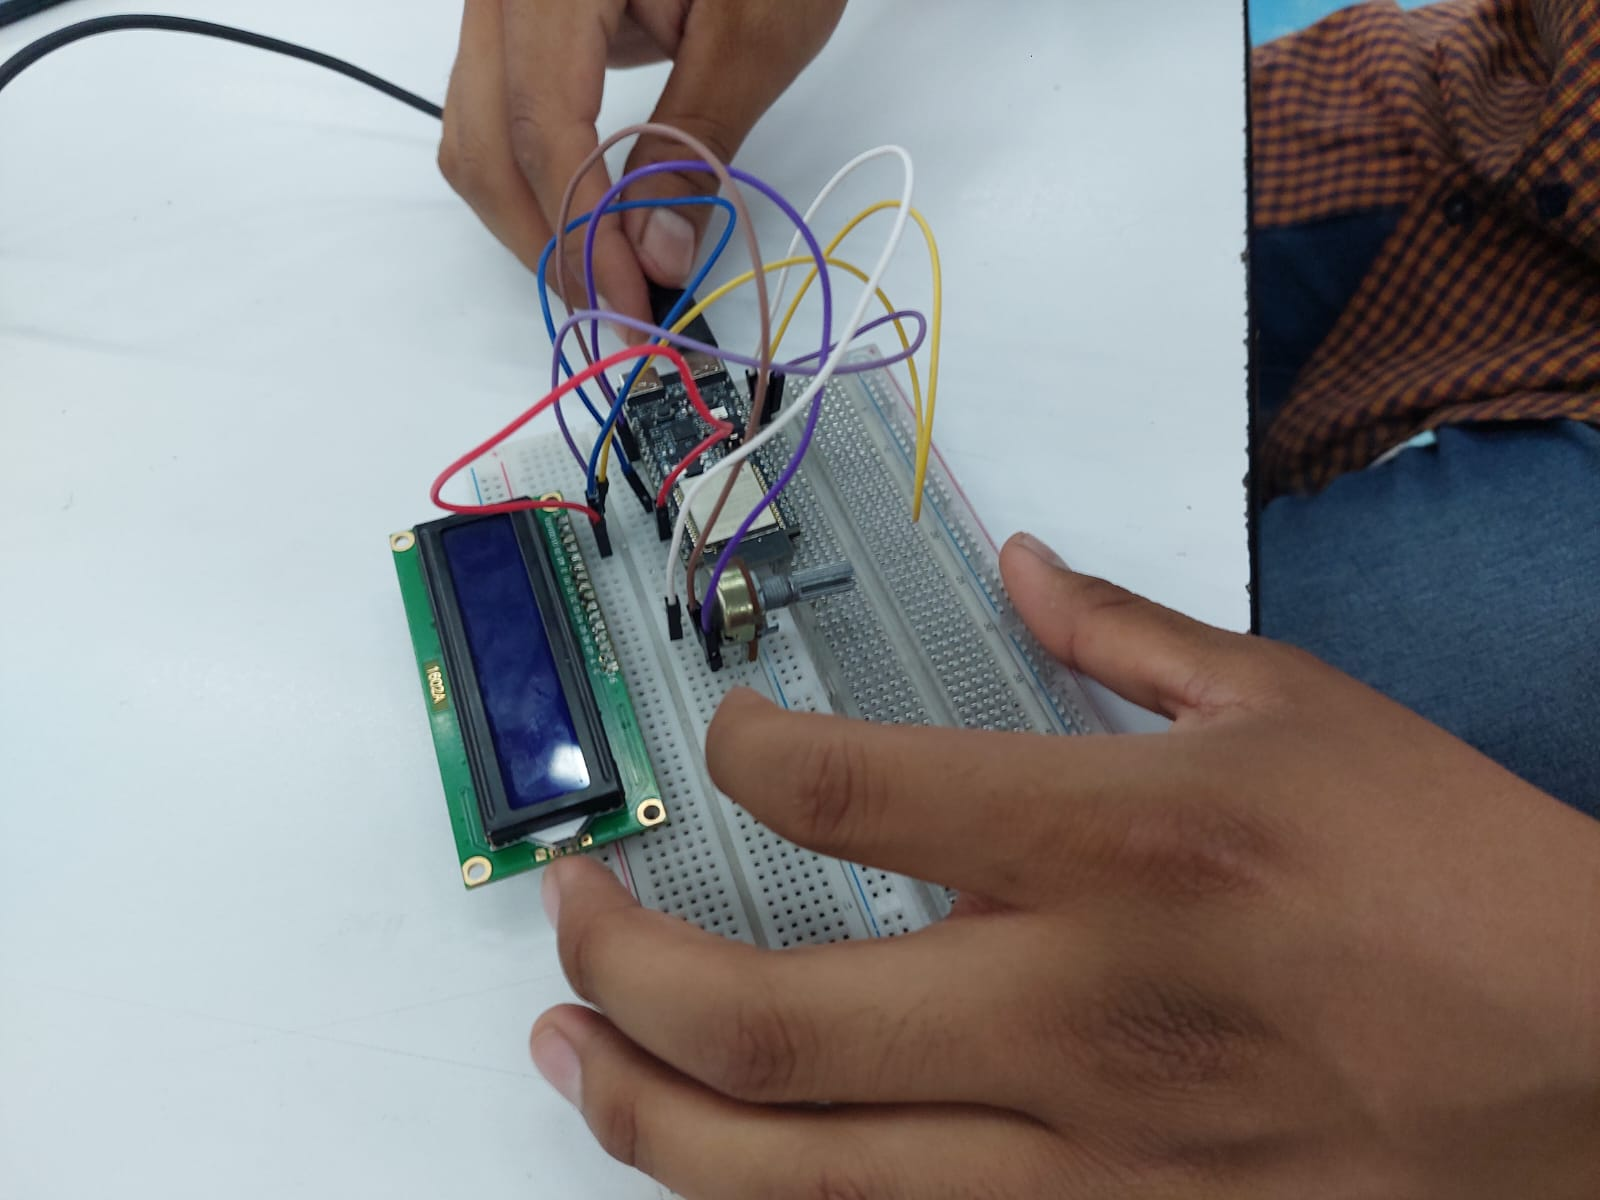
\includegraphics[trim = {0mm 0mm 0mm 0mm},clip,scale=0.2]{10/Img/muestra1Prueba3.jpg}
        \caption{Evidencia 3 de la primera muestra}
        \label{muestra1Prueba3}
    \end{figure}

\begin{figure}[H]
        \centering
        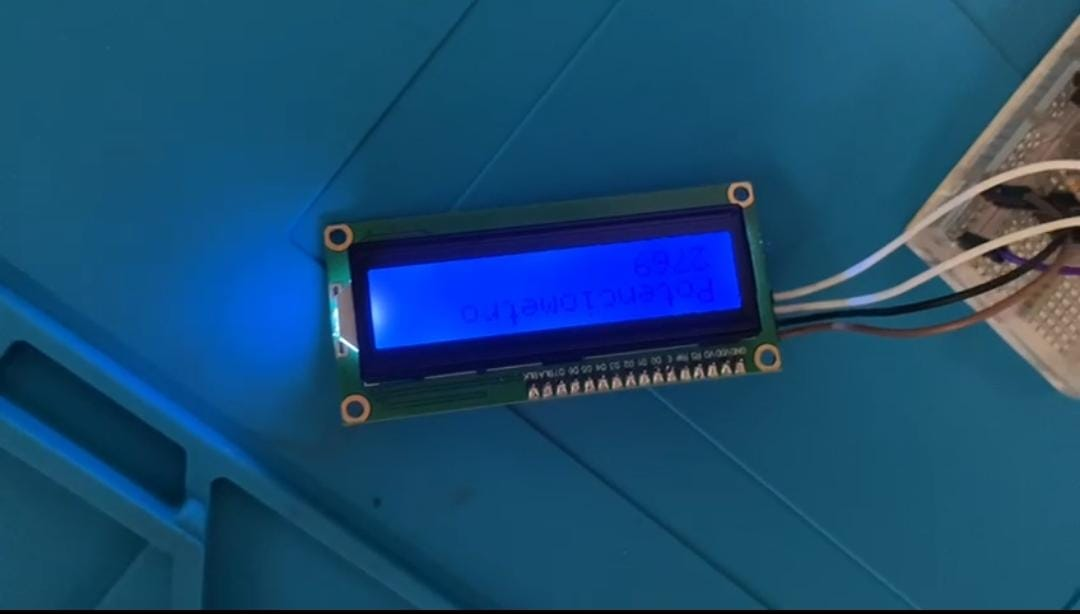
\includegraphics[trim = {0mm 0mm 0mm 0mm},clip,scale=0.2]{10/Img/muestra1Prueba4.jpg}
        \caption{Evidencia 4 de la primera muestra}
        \label{muestra1Prueba4}
    \end{figure}

Como se puede ver en la figura \ref{muestra1Prueba4}, se logra ver que cuando el operador mueve el potenciómetro los datos de la LCD van cambiando, por lo que, el ensamble se realizo de manera exitosa en la primera muestra.

\begin{figure}[H]
        \centering
        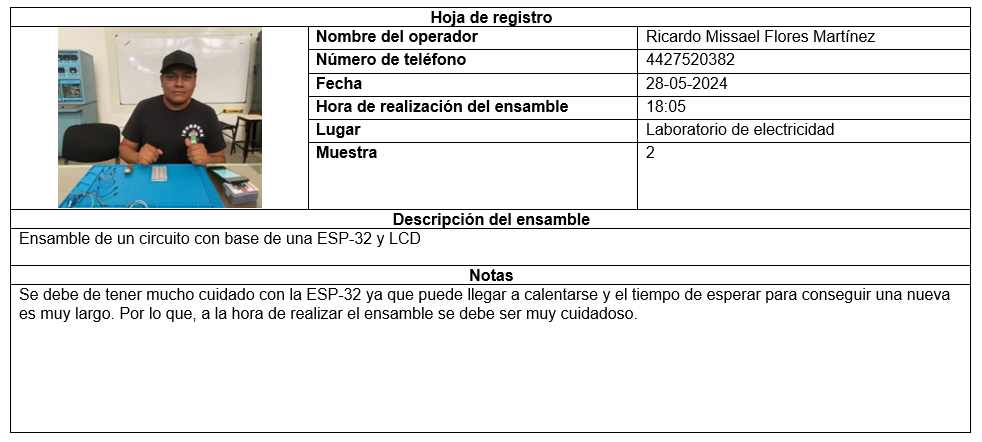
\includegraphics[trim = {0mm 0mm 0mm 0mm},clip,scale=0.2]{10/Img/hojaRegistro2.png}
        \caption{Hoja de registro de la segunda muestra}
        \label{hojaRegistro2}
    \end{figure}

\begin{figure}[H]
        \centering
        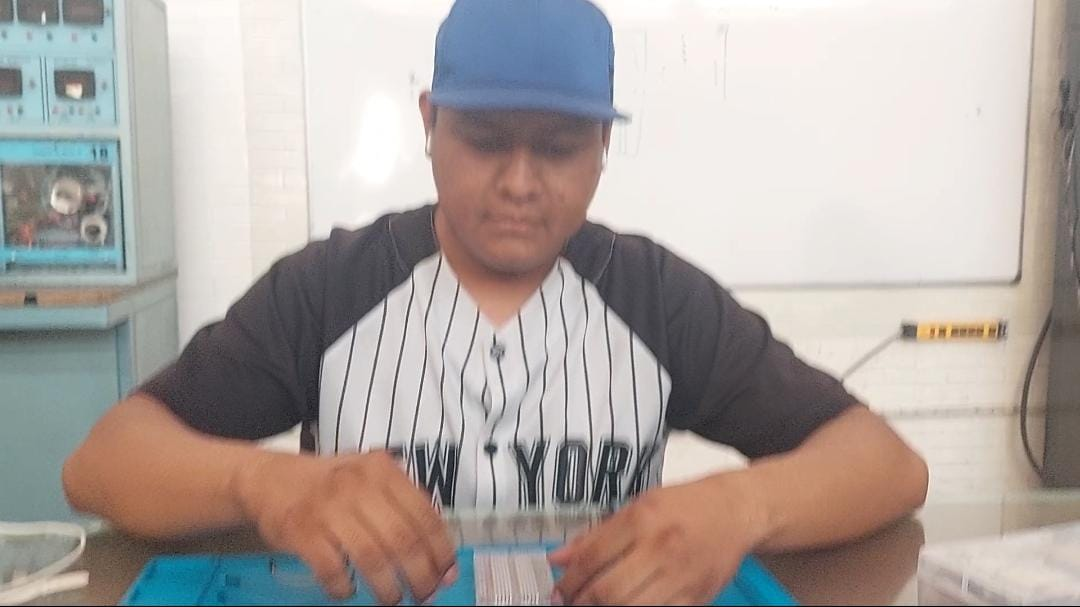
\includegraphics[trim = {0mm 0mm 0mm 0mm},clip,scale=0.2]{10/Img/muestra2Prueba1.jpg}
        \caption{Evidencia 1 de la segunda muestra}
        \label{muestra2Prueba1}
    \end{figure}

\begin{figure}[H]
        \centering
        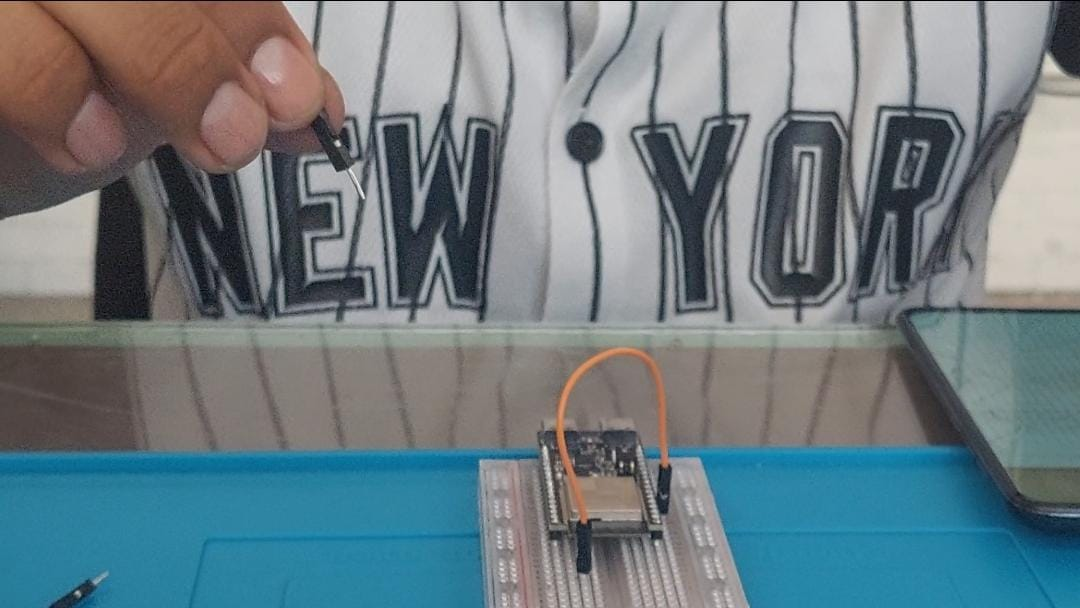
\includegraphics[trim = {0mm 0mm 0mm 0mm},clip,scale=0.2]{10/Img/muestra2Prueba2.jpg}
        \caption{Evidencia 2 de la segunda muestra}
        \label{muestra2Prueba2}
    \end{figure}

\begin{figure}[H]
        \centering
        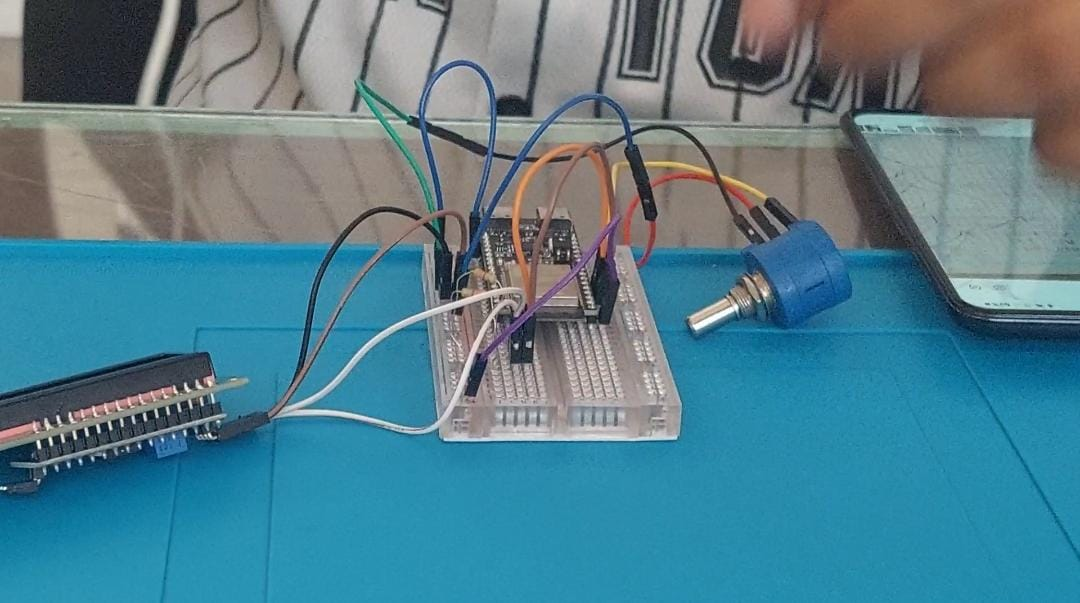
\includegraphics[trim = {0mm 0mm 0mm 0mm},clip,scale=0.2]{10/Img/muestra2Prueba3.jpg}
        \caption{Evidencia 3 de la segunda muestra}
        \label{muestra2Prueba3}
    \end{figure}

\begin{figure}[H]
        \centering
        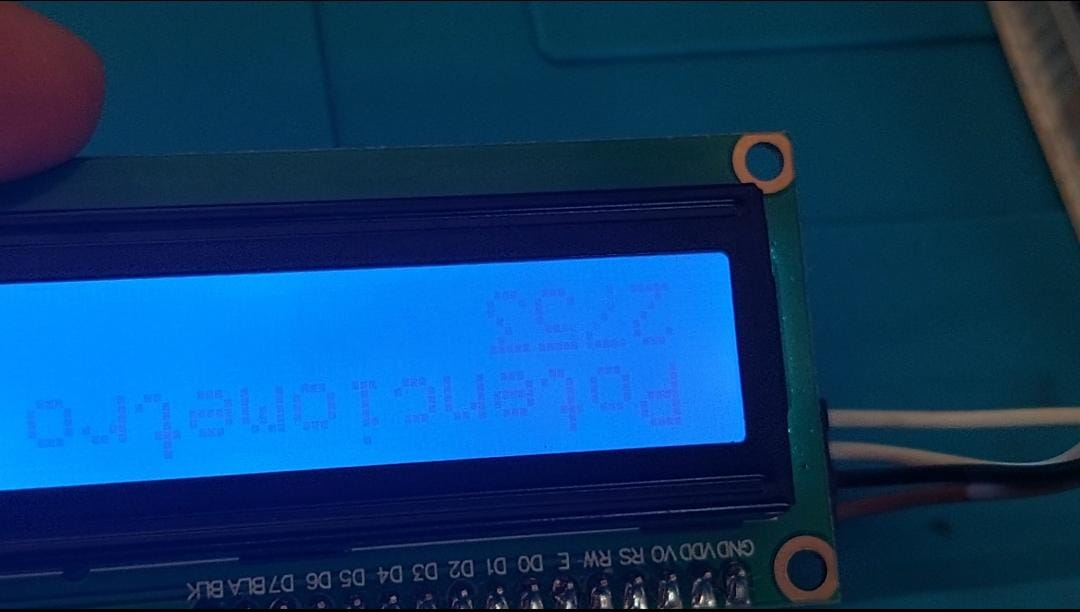
\includegraphics[trim = {0mm 0mm 0mm 0mm},clip,scale=0.2]{10/Img/muestra2Prueba4.jpg}
        \caption{Evidencia 4 de la segunda muestra}
        \label{muestra2Prueba4}
    \end{figure}
%
%
\subsubsection{Desarrollo del sistema de tiempos predeterminado}

\begin{figure}[H]
        \centering
        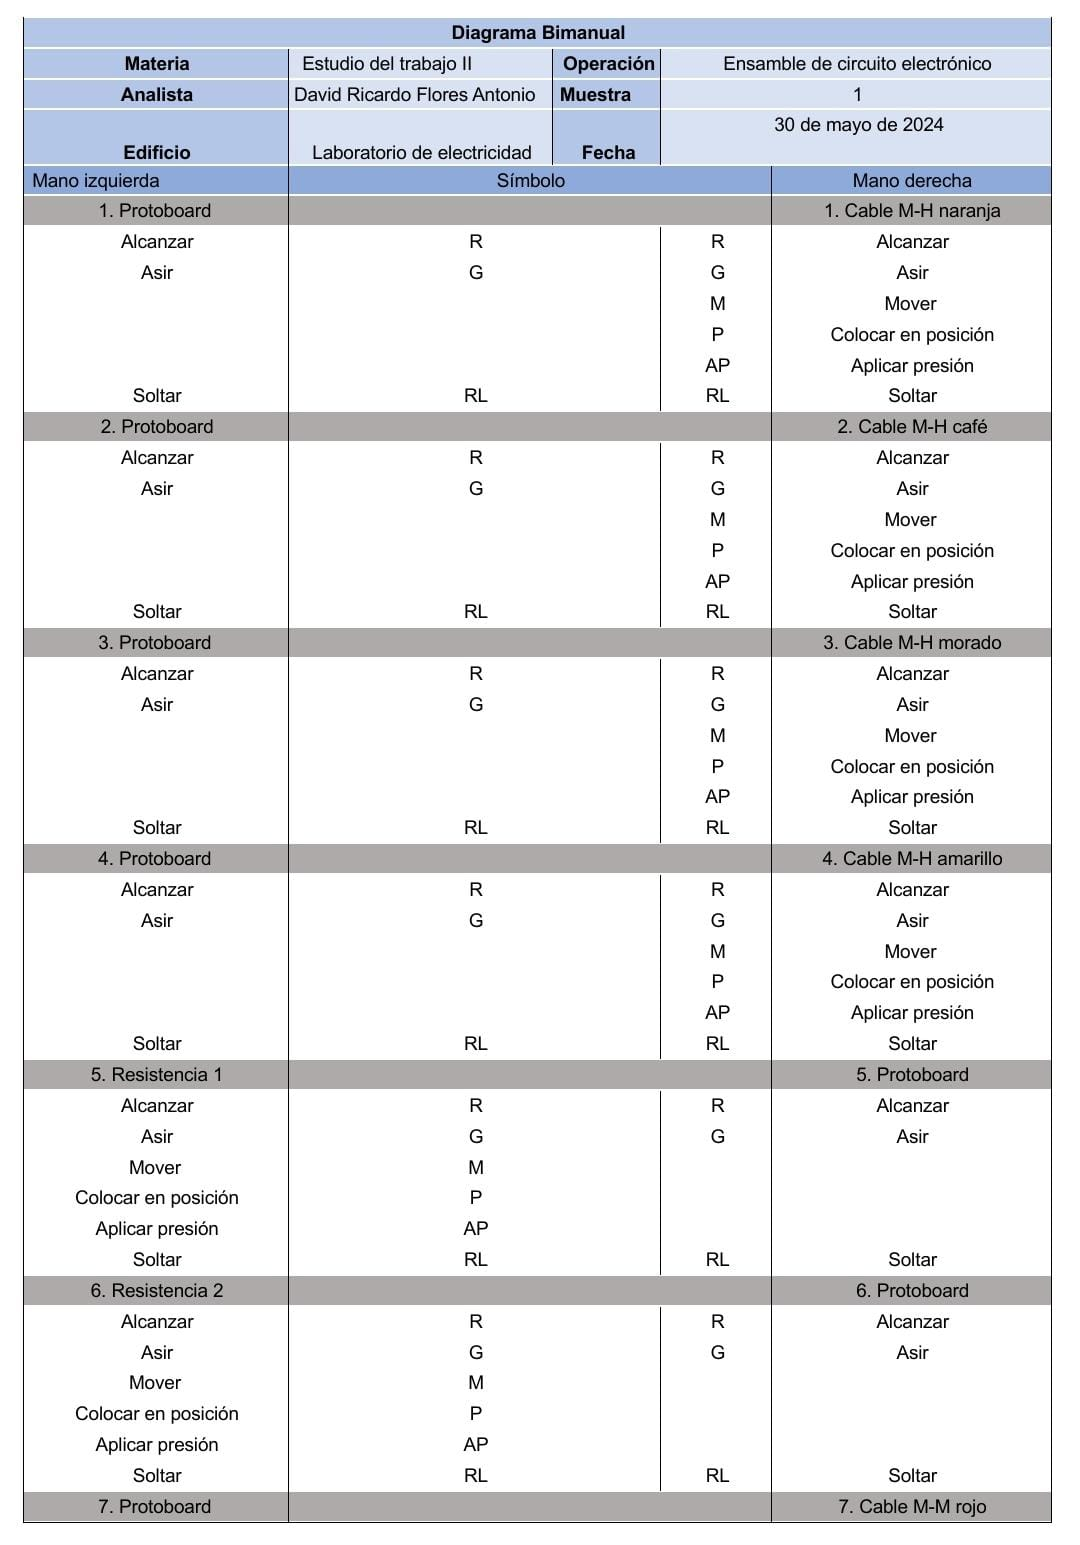
\includegraphics[trim = {0mm 0mm 0mm 0mm},clip,scale=0.2]{10/Img/diagramaBimanual1.jpg}
        \label{diagramaBimanual1}
    \end{figure}

\begin{figure}[H]
        \centering
        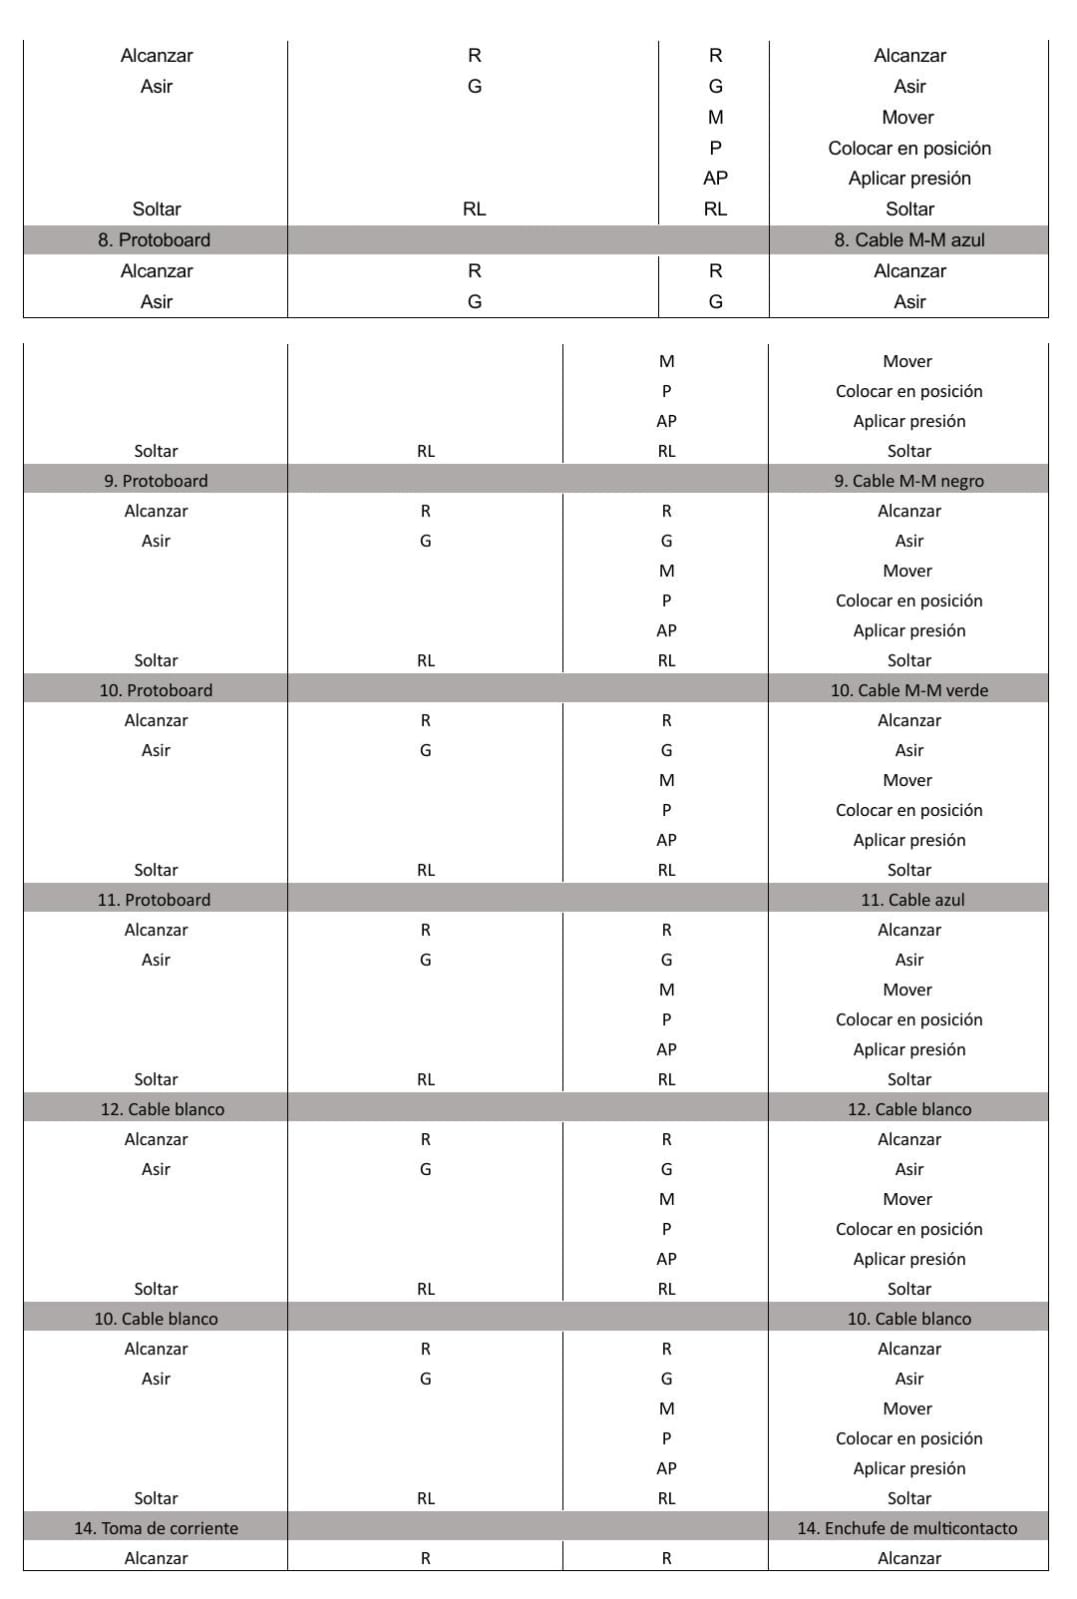
\includegraphics[trim = {0mm 0mm 0mm 0mm},clip,scale=0.2]{10/Img/diagramaBimanual2.jpg}
        \label{diagramaBimanual2}
    \end{figure}

\begin{figure}[H]
        \centering
        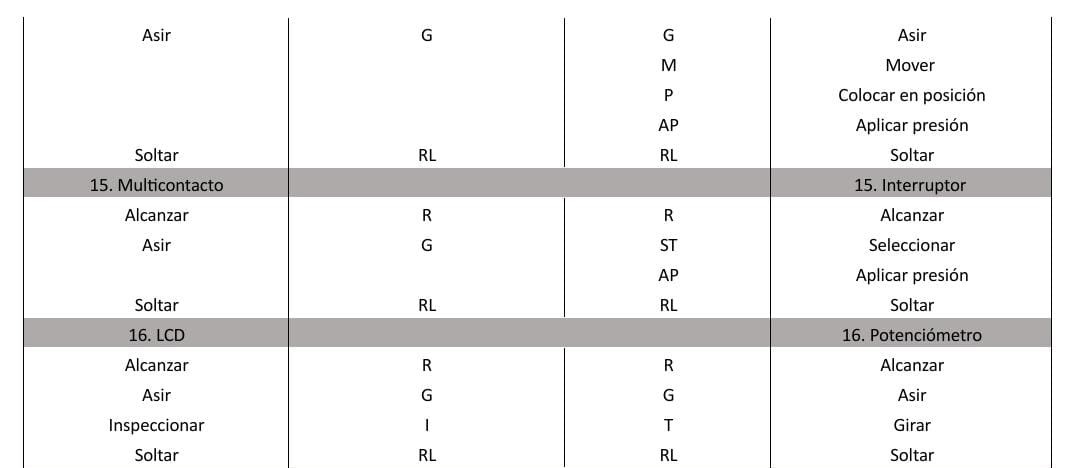
\includegraphics[trim = {0mm 0mm 0mm 0mm},clip,scale=0.2]{10/Img/diagramaBimanual3.jpg}
        \caption{Diagrama Bimanual}
        \label{diagramaBimanual3}
    \end{figure}
\subsubsection{Desarrollo del muestreo de trabajo}

\begin{figure}[H]
        \centering
        \includegraphics[trim = {0mm 0mm 0mm 0mm},clip,scale=0.4]{10/Img/tiempoEstándar.png}
        \caption{Tiempo ciclo}
        \label{tiempoEstándar}
    \end{figure}

\begin{figure}[H]
        \centering
        \includegraphics[trim = {0mm 0mm 0mm 0mm},clip,scale=0.4]{10/Img/muestreo1.png}
        \label{muestreo1}
    \end{figure}

\begin{figure}[H]
        \centering
        \includegraphics[trim = {0mm 0mm 0mm 0mm},clip,scale=0.4]{10/Img/muestreo2.png}
        \label{muestreo2}
    \end{figure}

\begin{figure}[H]
        \centering
        \includegraphics[trim = {0mm 0mm 0mm 0mm},clip,scale=0.4]{10/Img/muestreo3.png}
        \caption{Muestreo}
        \label{muestreo3}
    \end{figure}
La media de la variable aleatoria discreta (X) es:
\begin{equation}
     \mu_x=\dfrac{b+a}{2}
\end{equation}

La desviación estándar de X es:
\begin{equation}
     \sigma_x=\sqrt{\dfrac{(b-a+1)^2-1}{12}}
\end{equation}
\section{Conclusiones}
    
Al realizar las tomas de muestras, se obtuvo un tiempo de ciclo de 2.64 minutos. Estas muestras, mostradas en la tabla \ref{muestreo3}, permitieron determinar un tiempo estándar de 5.31 minutos e identificar al operador promedio y al más lento. Esto facilitó el balanceo de líneas y la reducción de tiempos con la ayuda de los therblings, lo que resultó en una producción balanceada y con costos operativos bajos. 
El propósito de este trabajo fue desarrollar un proyecto integrador mediante el ensamblaje de un circuito, aplicando todos los temas vistos a lo largo del semestre como estudio de movimientos y tiempos, muestras continuas o discretas, y conocimientos de otras materias como probabilidad y estadística, higiene y salud, y estudio del trabajo I.

El objetivo principal era diseñar, mejorar e integrar sistemas productivos de bienes y servicios, determinando el tiempo estándar en el ensamblaje del circuito. Sin embargo, el proyecto no se completó debido a complicaciones como retrasos con la ESP32. A pesar de esto, se aprendió mucho sobre la normalización de procesos a nivel profesional y la integración de conocimientos de distintas materias.

Se diseñó un ensamblaje electrónico y se creó un manual para capacitar a operarios sin experiencia. A través de dos pruebas de ensamblaje, se realizaron análisis para optimizar y reducir costos. Se usaron herramientas como Overleaf, GitHub y Visual Studio, ganando experiencia con tecnologías industriales.

El trabajo permitió obtener un tiempo estándar basado en los ciclos de las actividades del ensamblaje y múltiples mediciones de tiempos de distintos operarios. Aunque el proyecto no se terminó, se alcanzaron la mayoría de los objetivos y se cubrió casi completamente la hipótesis, proporcionando una valiosa experiencia para futuros trabajos como ingenieros industriales.

    \section{Agradecimientos}
    
Quisiera expresar mi más sincero agradecimiento a todas las personas y organizaciones que han contribuido al desarrollo de este proyecto.

En primer lugar, agradezco a mi profesor de Estudio del Trabajo II por su orientación y apoyo constante. Su conocimiento y experiencia fueron fundamentales para la realización de este trabajo.

También quiero agradecer a mis compañeros de grupo, por su dedicación, colaboración y esfuerzo. Su compromiso fue clave para superar los desafíos que encontramos en el camino.

Agradezco al Instituto Tecnológico de Querétaro por brindarnos los recursos y el entorno adecuado para llevar a cabo este proyecto. Sin su apoyo, no habría sido posible lograr nuestros objetivos.

    
%\section{Referencias}
    
  %  Para esta platilla, se solicita al autor enumerar las citas de manera consecutiva entre corchetes 
   % La puntuación de la oración que sigues sería  
   % Refiérase simplemente al número de referencia, como en , no utilice “Ref. [3]” o “referencia [3]” excepto al principio de una oración: “La referencia [3] fue la primera…”
   % Enumere las notas al pie por separado en superíndices. Coloque la nota de pie de en la parte inferior de la columna en la que se citó. No coloque notas al pie en la lista de referencias. Utilice letras para las notas al pie de la tabla.
   % A menos de que haya tres autores o más; no utilice “et al.”. Los trabajos que no hayan sido publicados, incluso si han sido presentados para su publicación, deben ser citados como “inéditos”. Los trabajos que han sido aceptados para su publicación deben de citarse como “en prensa”. Poner en mayúscula sólo la primera palabra de un %título, excepto los nombres propios y los símbolos de %elemento. 
    %Otros ejemplos 
    %Véase el link  Véase el Apéndice 
    
    % Ejemplo
    %  @Article{article,
    % 	author = "Author1 LastName1 and Author2 LastName2 and Author3 LastName3",
    % 	title = "Article Title",
    % 	volume = "30",
    % 	number = "30",
    % 	pages = "10127-10134",
    % 	year = "2013",
    % 	doi = "10.3389/fnins.2013.12345",
    % 	URL = "http://www.frontiersin.org/Journal/10.3389/fnins.2013.12345/abstract",
    % 	journal = "Frontiers in Neuroscience"
    % }
    
    % @book{book,
    %   author    = {Author Name}, 
    %   title     = {The title of the work},
    %   publisher = {The name of the publisher},
    %   address   = {The city},
    %   year      = 1993,
    % }
    
    % @incollection{chapter,
    %   author       = {Bauthor Surname}, 
    %   title        = {The title of the work},
    %   editor       = {Editor Name},
    %   booktitle    = {The title of the book},
    %   publisher    = {The name of the publisher},
    %   address      = {The city},
    %   year         = 2002,
    %   pages        = {201-213},
    % }
    
    % @InProceedings{conference,
    %   author = {Cauthor Name and Dauthor Surname and Fauthor LastName},
    %   title = {The title of the work},
    %   booktitle = {The title of the conference proceedings},
    %   year = 1996,
    %   publisher = {The name of the publisher},
    %   editor = {Editor Name1 and Editor Name2},
    %   pages = {41-50},
    % }
    
    % @book{cho,
    %   author       = {Gauthor Name1}, 
    %   title        = {The title of the work},
    %   publisher = {Country code and patent number},
    %   address      = {Patent Country},
    %   year = 2013
    % }
    
    % @book{patent,
    %   author    = {Hauthor Surname1}, 
    %   title     = {The title of the work},
    %   publisher = {Patent number},
    %   address   = {Patent country},
    %   year      = 2010,
    % }
    
    % % please use misc for datasets
    % @misc{dataset, 
    % 	author = "Author1 LastName1 and Author2 LastName2 and Author3 LastName3",
    % 	title = "Data Title",
    % 	year = "2011",
    % 	doi = "10.000/55555",
    % 	URL = "http://www.frontiersin.org/",
    % }
    \bibliographystyle{ieeetr}
    \bibliography{10/referencias}
    % 
    % 
    %%%%%%%%%%%%%%%%%%%%%%%%%%%%%%%%%%
   \newpage
   \appendix
   %%%%%%%%%%%%%%%%%%%%%%%%%%%%%%%%%%
   %
   %
   \centering{\section[\appendixautorefname{}]{APÉNDICE}}\label{anexo:manualOperador}
    \includepdf[pages=-]{10/Img/manualOperador.pdf}
    %%%%%%%%%%%%%%%%%%%%%%%%%%%%%%%%%%%%%%%%%